% \documentclass[aspectratio=169,notes]{beamer}
\documentclass[aspectratio=169]{beamer}
\usetheme[faculty=phil]{fibeamer}
\usepackage{polyglossia}
\setmainlanguage{english} %% main locale instead of `english`, you
%% can typeset the presentation in either Czech or Slovak,
%% respectively.
\setotherlanguages{russian} %% The additional keys allow
%%
%%   \begin{otherlanguage}{czech}   ... \end{otherlanguage}
%%   \begin{otherlanguage}{slovak}  ... \end{otherlanguage}
%%
%% These macros specify information about the presentation
\title[Artificial Intelligence Software (AIS)]{Artificial Intelligence Software, Lecture 4} %% that will be typeset on the
\subtitle{Data preprocessing
\\ \ \\ \  } %% title page.
\author{Oleg Bulichev}
%% These additional packages are used within the document:
\usepackage{ragged2e}  % `\justifying` text
\usepackage{booktabs}  % Tables
\usepackage{tabularx}
\usepackage{tikz}      % Diagrams
\usetikzlibrary{calc, shapes, backgrounds}
\usetikzlibrary{decorations.pathreplacing,calligraphy,calc,graphs}
\usepackage{amsmath, amssymb}
\usepackage{url}       % `\url`s
\usepackage{listings}  % Code listings
\usepackage{subfigure}
% \usepackage{floatrow}
% \usepackage{subcaption}
\usepackage{mathtools}
\usepackage{todonotes}
\usepackage{fontspec}
\usepackage{multicol}
\usepackage{pdfpages}
\usepackage{wrapfig}
\usepackage{qrcode}
\usepackage{animate}
\usepackage{booktabs}
\usepackage{multirow}
\usepackage{graphicx}
\usepackage{colortbl}

\graphicspath{{resources/}}
\frenchspacing

\setbeamertemplate{caption}{\raggedright\insertcaption\par}
\usetikzlibrary{graphs}

% \usepackage[backend=biber,style=ieee,autocite=footnote]{biblatex}
% \addbibresource{biblio.bib}
% \DefineBibliographyStrings{english}{%
%   bibliography = {References},}

\newcommand{\oleg}[2][] {\todo[color=red, #1] {OLEG:\\ #2}}
\newcommand{\fbckg}[1]{\usebackgroundtemplate{\includegraphics[width=\paperwidth]{#1}}}%frame background

\usepackage[framemethod=TikZ]{mdframed}
\newcommand{\dbox}[1]{
\begin{mdframed}[roundcorner=3pt, backgroundcolor=yellow, linewidth=0]
\vspace{1mm}
{#1}
\vspace{1mm}
\end{mdframed}
}

\begin{document}
\setlength{\abovedisplayskip}{0pt}
\setlength{\belowdisplayskip}{0pt}
\setlength{\abovedisplayshortskip}{0pt}
\setlength{\belowdisplayshortskip}{0pt}

\fbckg{fibeamer/figs/title_page.png}
\frame[c]{\setcounter{framenumber}{0}
    \usebeamerfont{title}%
    \usebeamercolor[fg]{title}%
    \begin{minipage}[b][6.5\baselineskip][b]{\textwidth}%
        \textcolor{black}{\raggedright\inserttitle}
    \end{minipage}
    % \vskip-1.5\baselineskip

    \usebeamerfont{subtitle}%
    \usebeamercolor[fg]{framesubtitle}%
    \begin{minipage}[b][3\baselineskip][b]{\textwidth}
        \raggedright%
        \insertsubtitle%
    \end{minipage}
    \vskip.25\baselineskip
}
%   \frame[c]{\maketitle}

\fbckg{fibeamer/figs/common.png}

\note{\scriptsize \begin{itemize}
        \item \
    \end{itemize}}


% --- BLOCK 1: WHY DATA PROCESSING MATTERS ---
\begin{frame}[t]{Outline}
\framesubtitle{}
    \vspace*{-0.5cm}
    \tableofcontents[hideallsubsections]
\end{frame}

\begin{frame}[t]{Reference materials}
\framesubtitle{}
\begin{figure}[H]
    \centering
\includegraphics[height=6cm,width=1\textwidth,keepaspectratio]{ref_data.png}
    \label{fig:ref_data.png}
\end{figure}
\end{frame}

\section{Importance of Data Processing}

\begin{frame}[t]{Concept: Garbage In, Garbage Out (GIGO)}
    \begin{columns}[T,onlytextwidth]
        \begin{column}{0.49\textwidth}
    \begin{itemize}
        \item Data is rarely ready for analysis in its raw form.
        \item 80\% of an analyst's time is spent on data preparation.
        \item Models are only as good as the data they consume.
    \end{itemize}
    \vspace{0.5cm}
    \textbf{Principle:} Quality over Complexity.
        \end{column}
        \begin{column}{0.49\textwidth}
            \vspace*{-0.4cm}
            \begin{figure}[H]
                \centering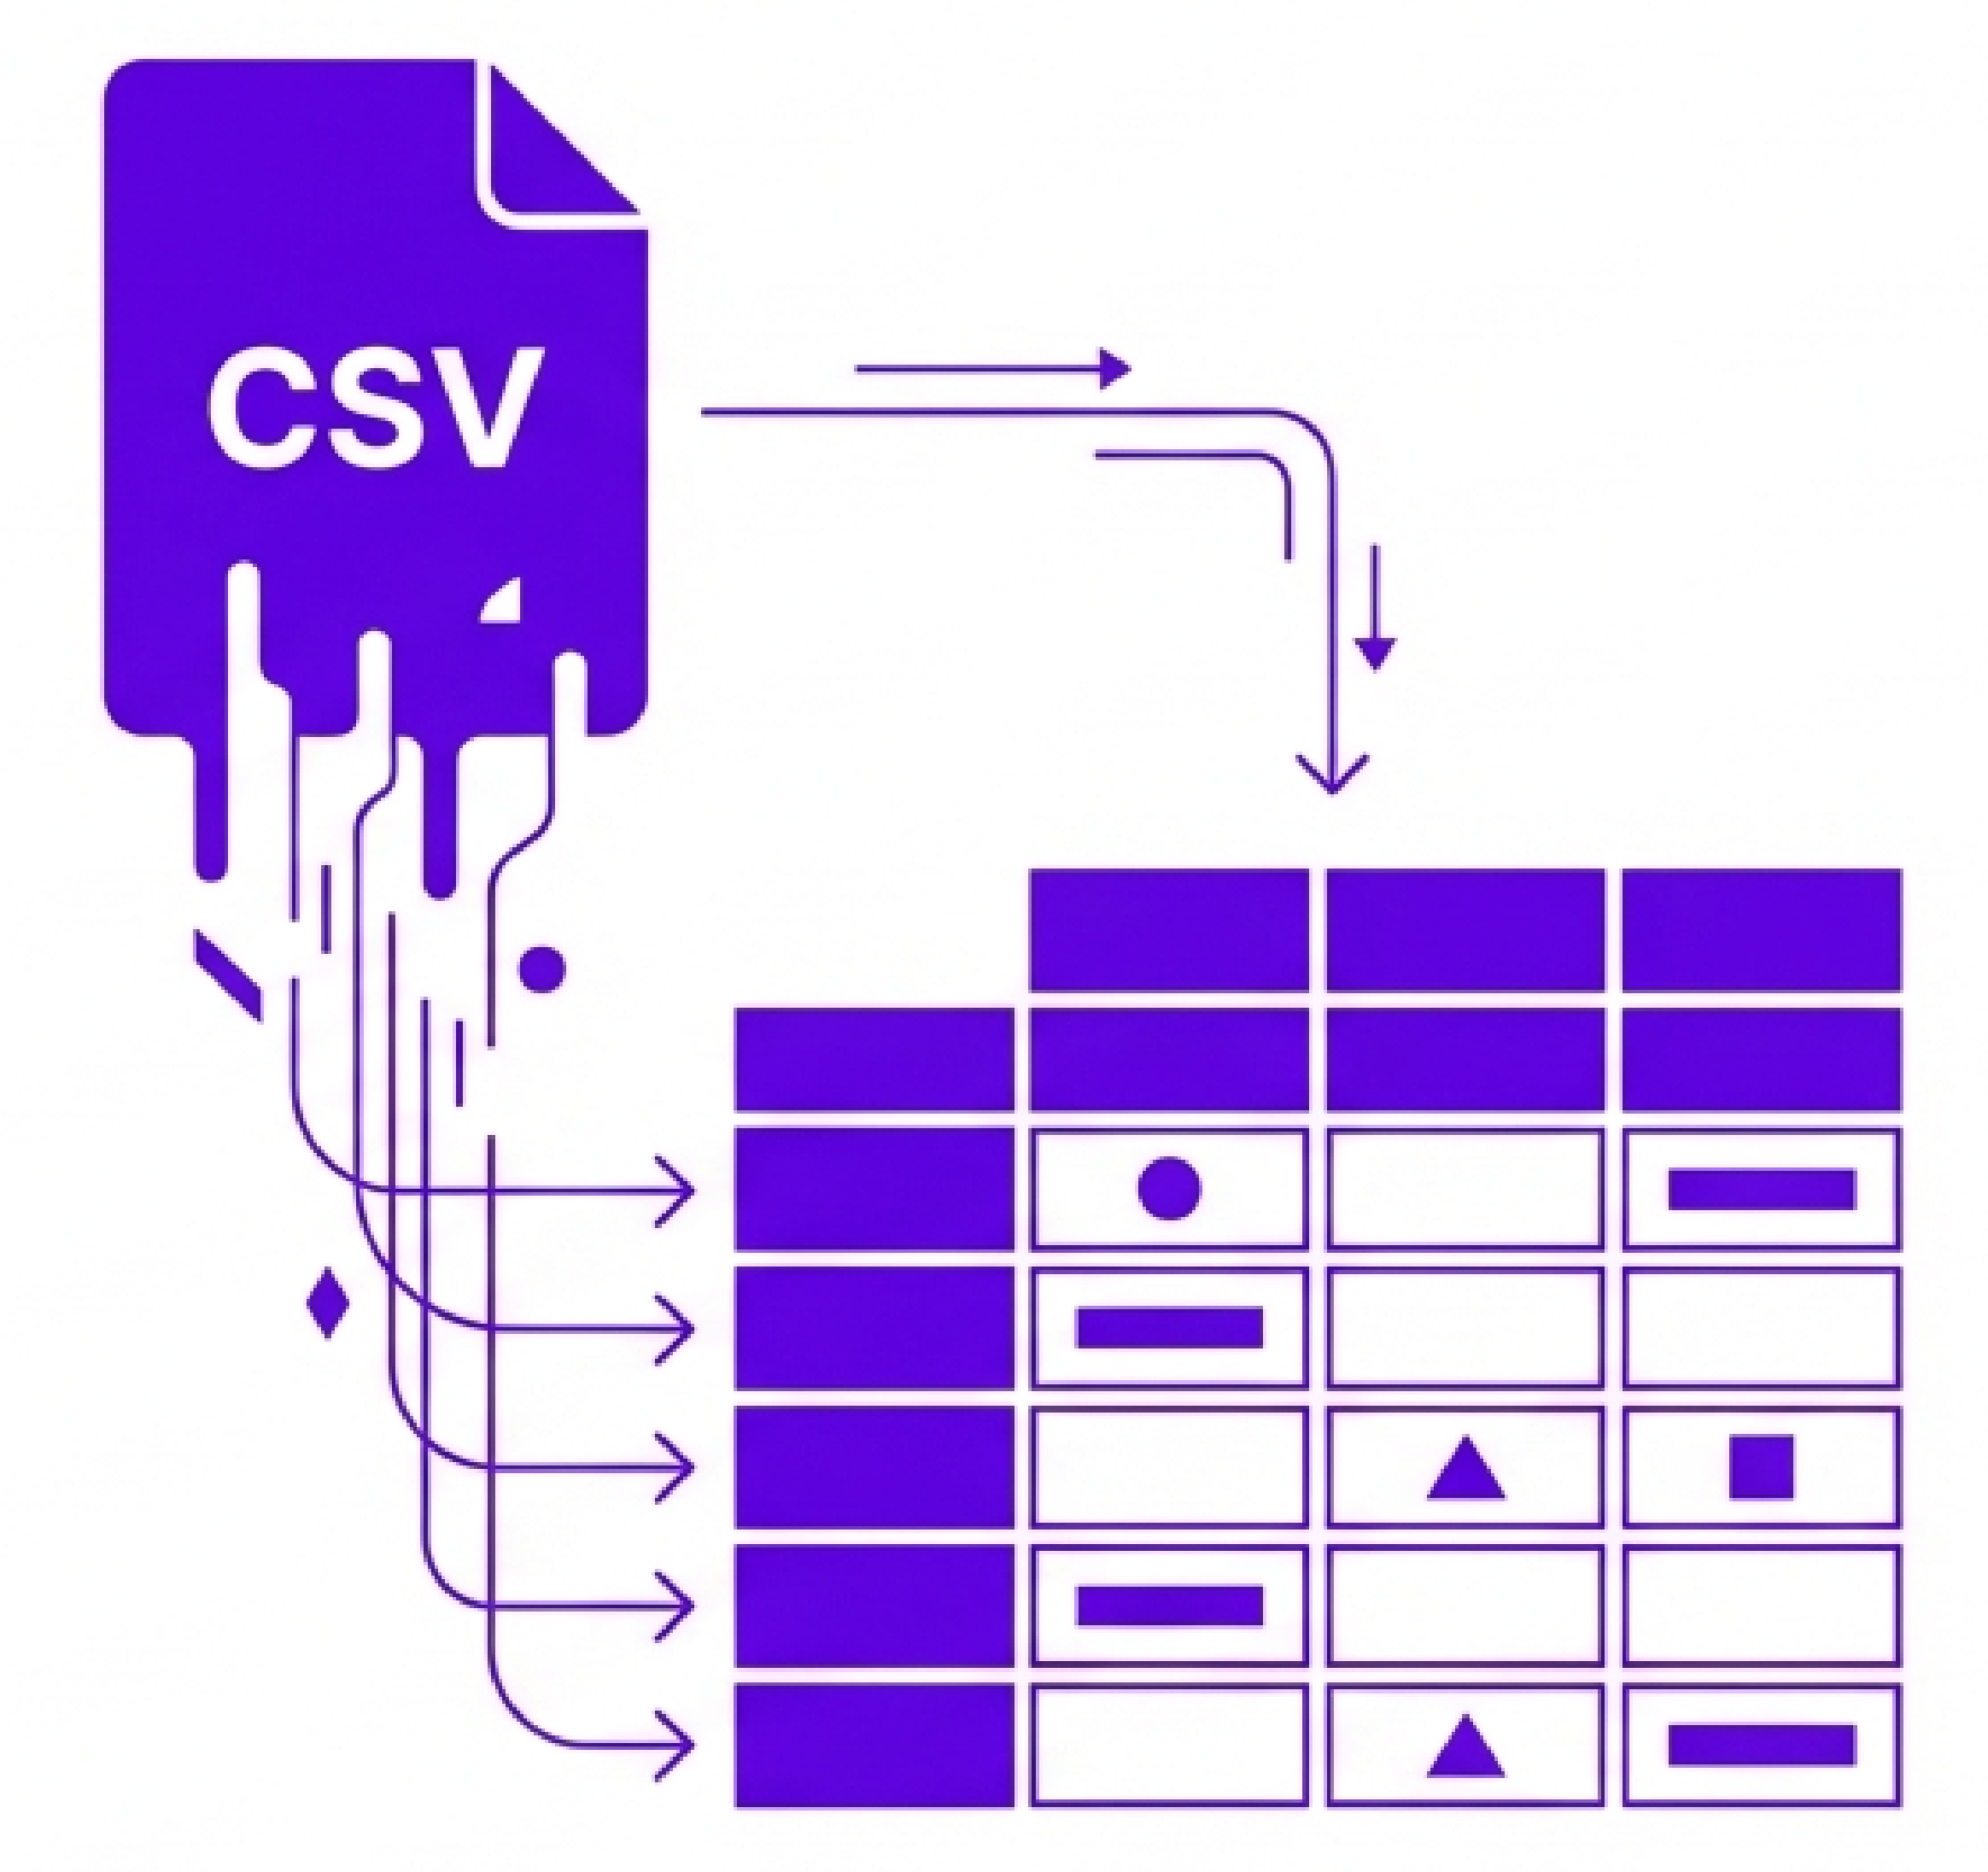
\includegraphics[height=6cm,width=1\textwidth,keepaspectratio]{csv_to_data.png}
                % \caption{caption_name}
                \label{fig:csv_to_data.png}
            \end{figure}
        \end{column}
    \end{columns}
    \note{Покажите визуальную абстракцию из источника: как CSV превращается в структурированную таблицу. Это первый шаг мышления аналитика [1].}
\end{frame}

\begin{frame}[t]{Example: The Titanic Objective}
    \vspace*{-0.5cm}
    \begin{figure}[H]
        \centering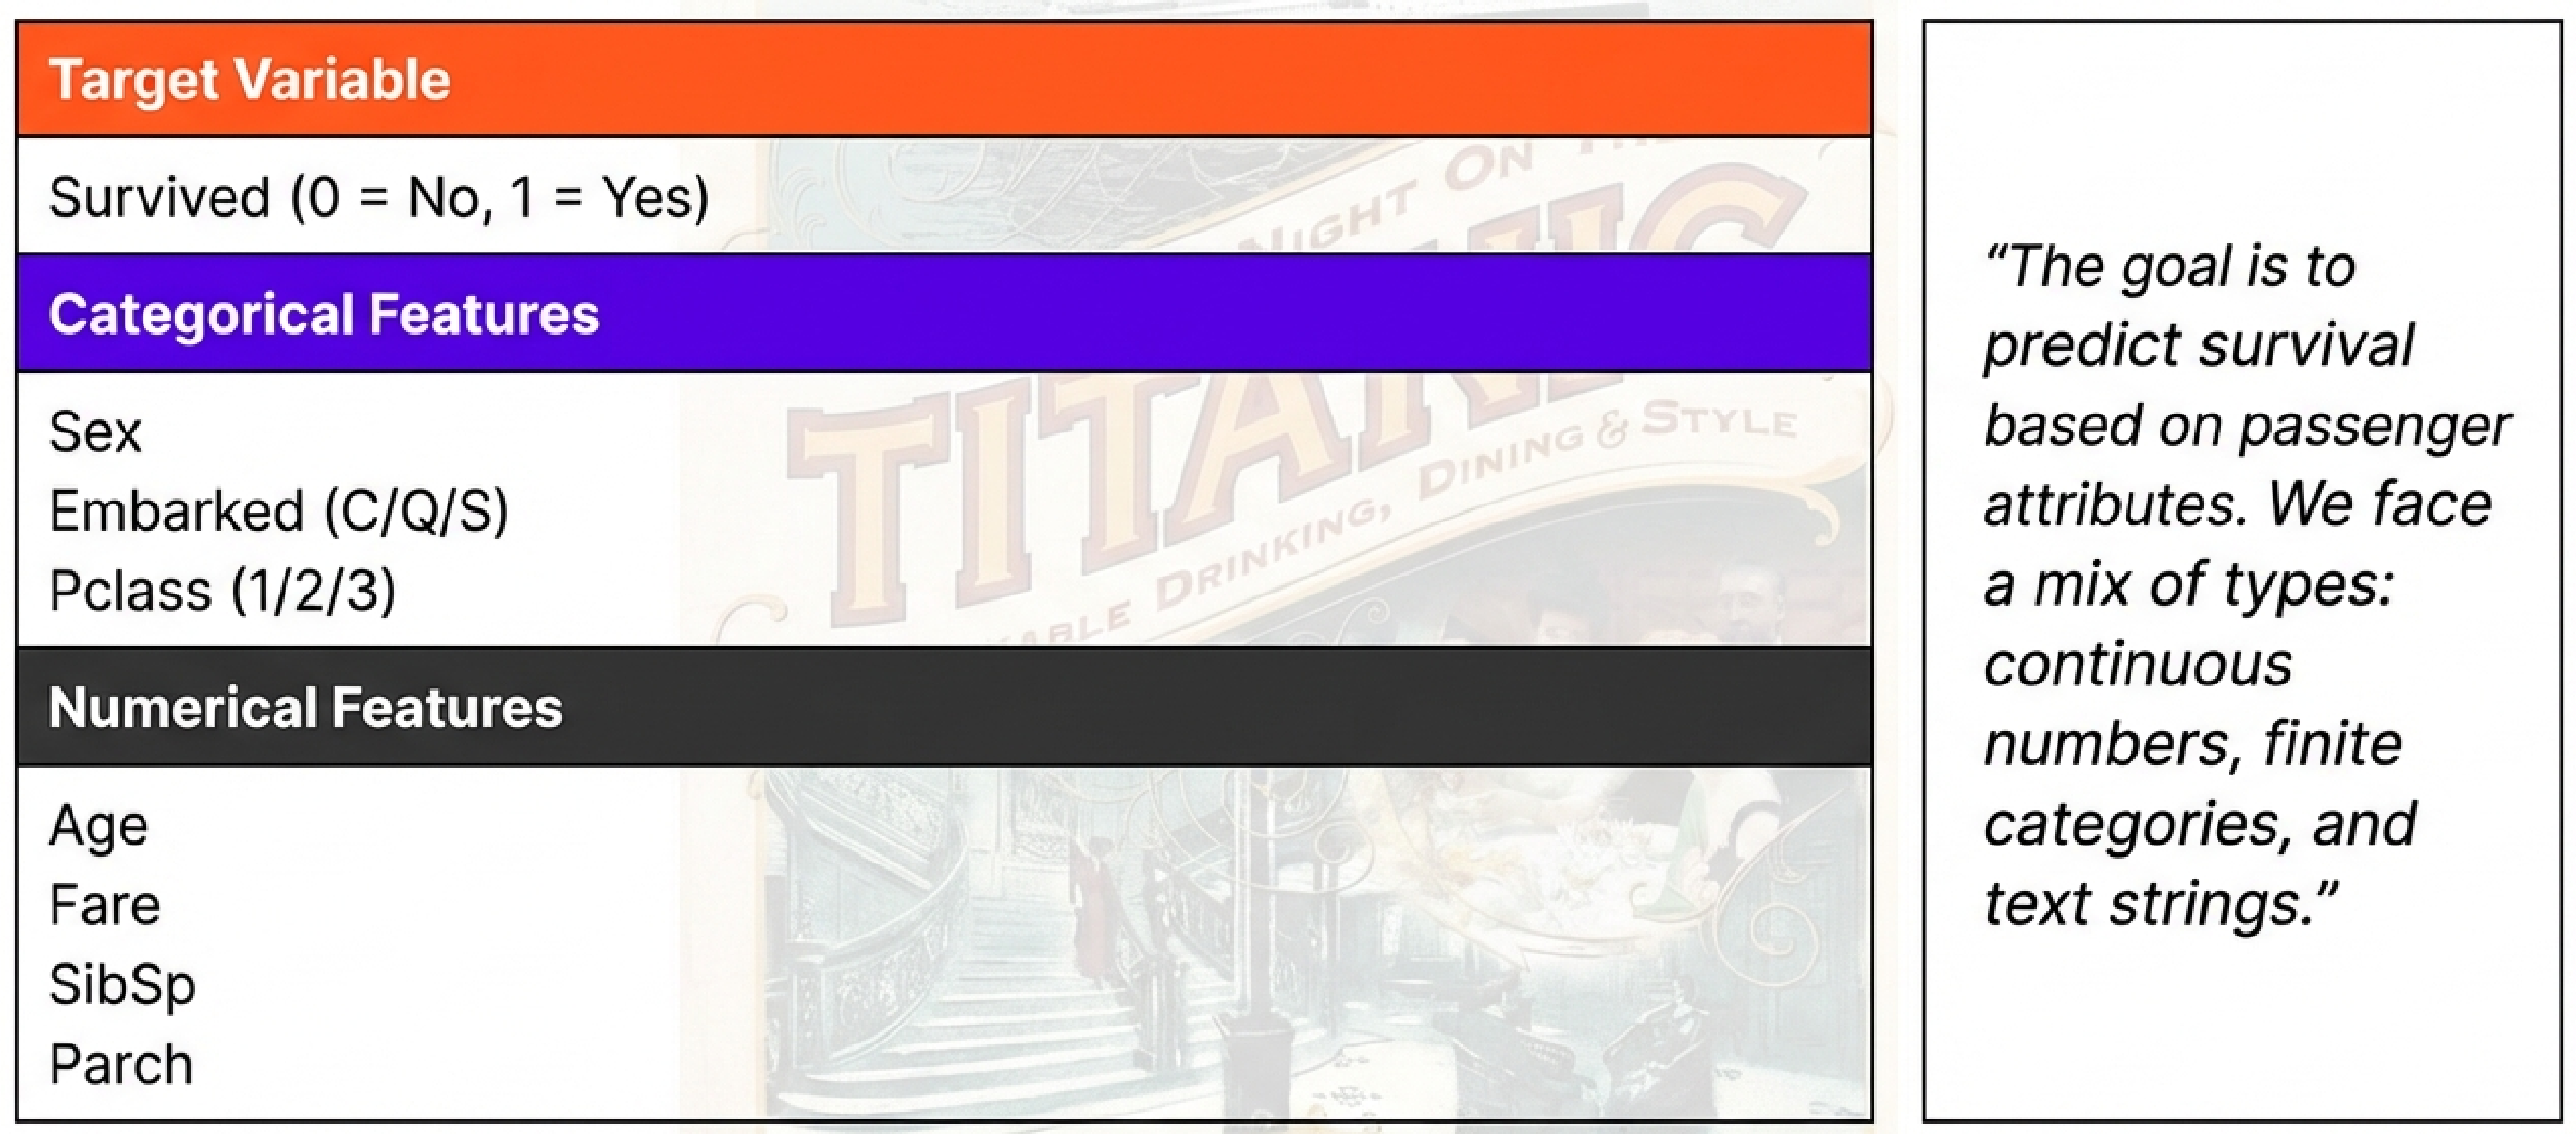
\includegraphics[height=6cm,width=1\textwidth,keepaspectratio]{objective.png}
        % \caption{caption_name}
        \label{fig:objective.png}
    \end{figure}
    \note{Используйте таблицу из материалов, чтобы показать разделение на целевую переменную (Survived) и разные типы признаков (Sex, Age, Pclass) [2].}
\end{frame}

\begin{frame}[t]{The Analytical Pipeline}
    \begin{figure}[H]
        \centering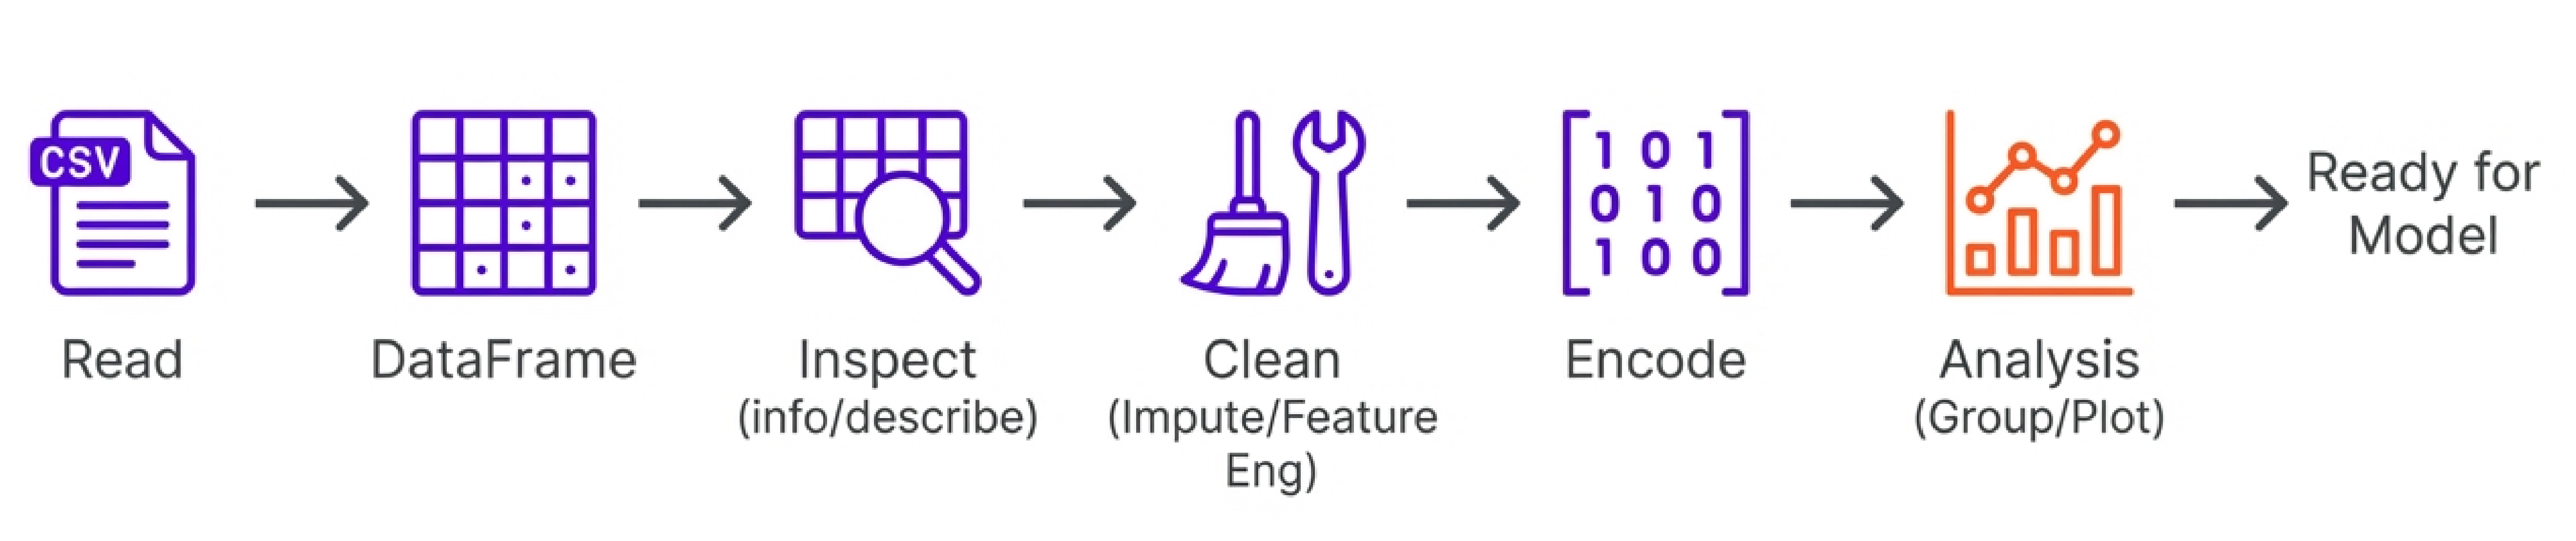
\includegraphics[height=6cm,width=1\textwidth,keepaspectratio]{data_workflow.png}
        % \caption{caption_name}
        \label{fig:data_workflow.png}
    \end{figure}
    \note{Краткий обзор пайплайна. Это карта нашего сегодняшнего занятия.}
\end{frame}

\begin{frame}[t]{Where to Study}
    \begin{itemize}
        \item \textbf{Wes McKinney PDF:} Chapter 1 "Preliminaries" (Page 24).
        \item \textbf{Video:} \href{https://www.youtube.com/watch?v=cqBTDb4un-Q}{"Introduction to Data Analysis. Part 1" (Intro section).}
    \end{itemize}
    \note{Дайте ссылки на материалы. Глава 1 Уэса Маккинни объясняет философию инструментов Python как «клея» для данных [12].}
\end{frame}

% --- BLOCK 2: TABULAR THINKING ---
\section{Tabular Thinking}

\begin{frame}[t]{Pandas Data Structures}
    \vspace*{-0.5cm}
    \begin{figure}[H]
        \centering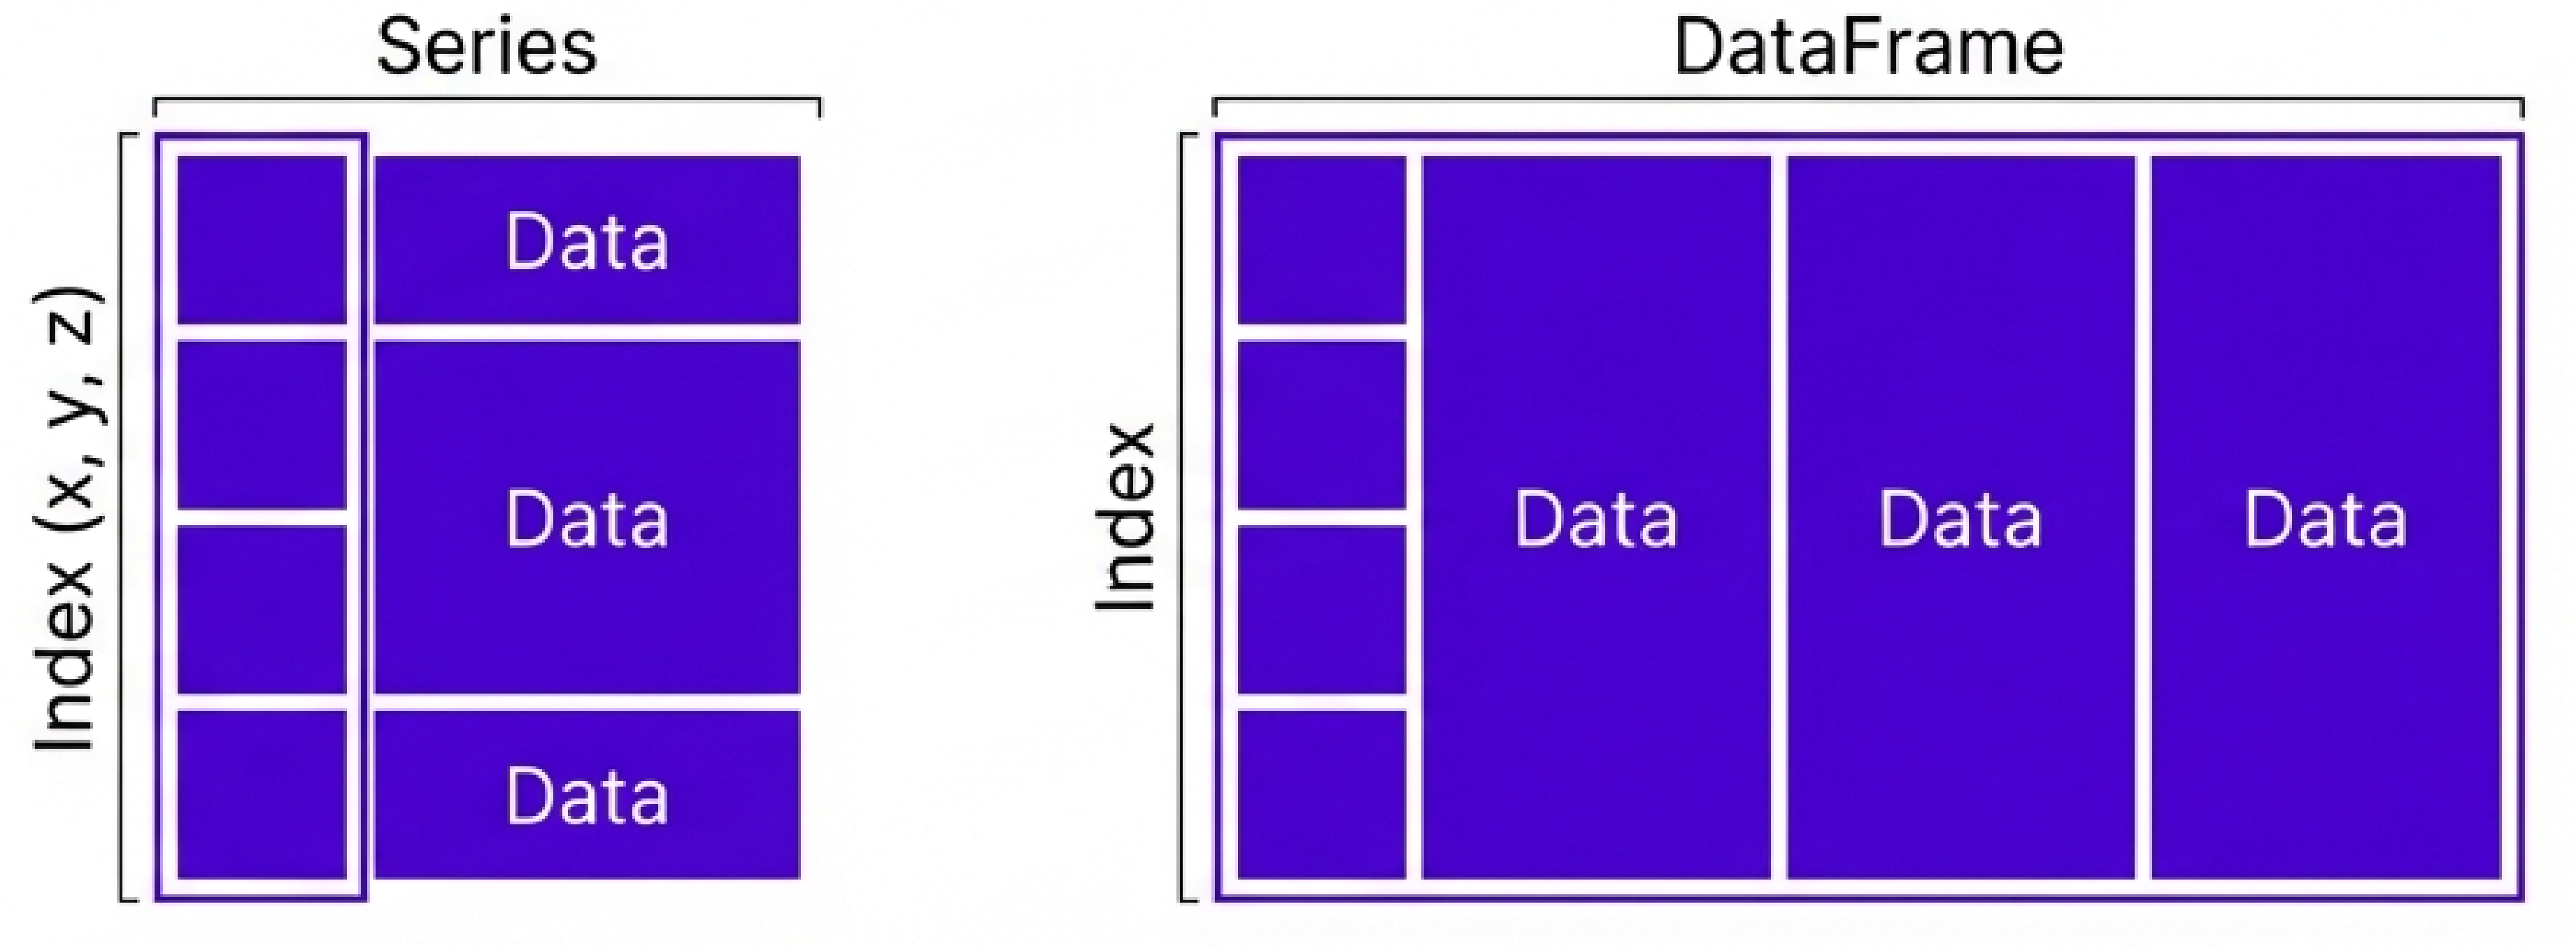
\includegraphics[height=5cm,width=1\textwidth,keepaspectratio]{dataframe.png}
        % \caption{caption_name}
        \label{fig:dataframe.png}
    \end{figure}
    \note{Объясните разницу между одномерным Series и двумерным DataFrame, используя наглядную схему из слайдов [3].}
\end{frame}


\begin{frame}[t]{Data Inspection Tools}
    \vspace*{-0.5cm}
    \begin{figure}[H]
        \centering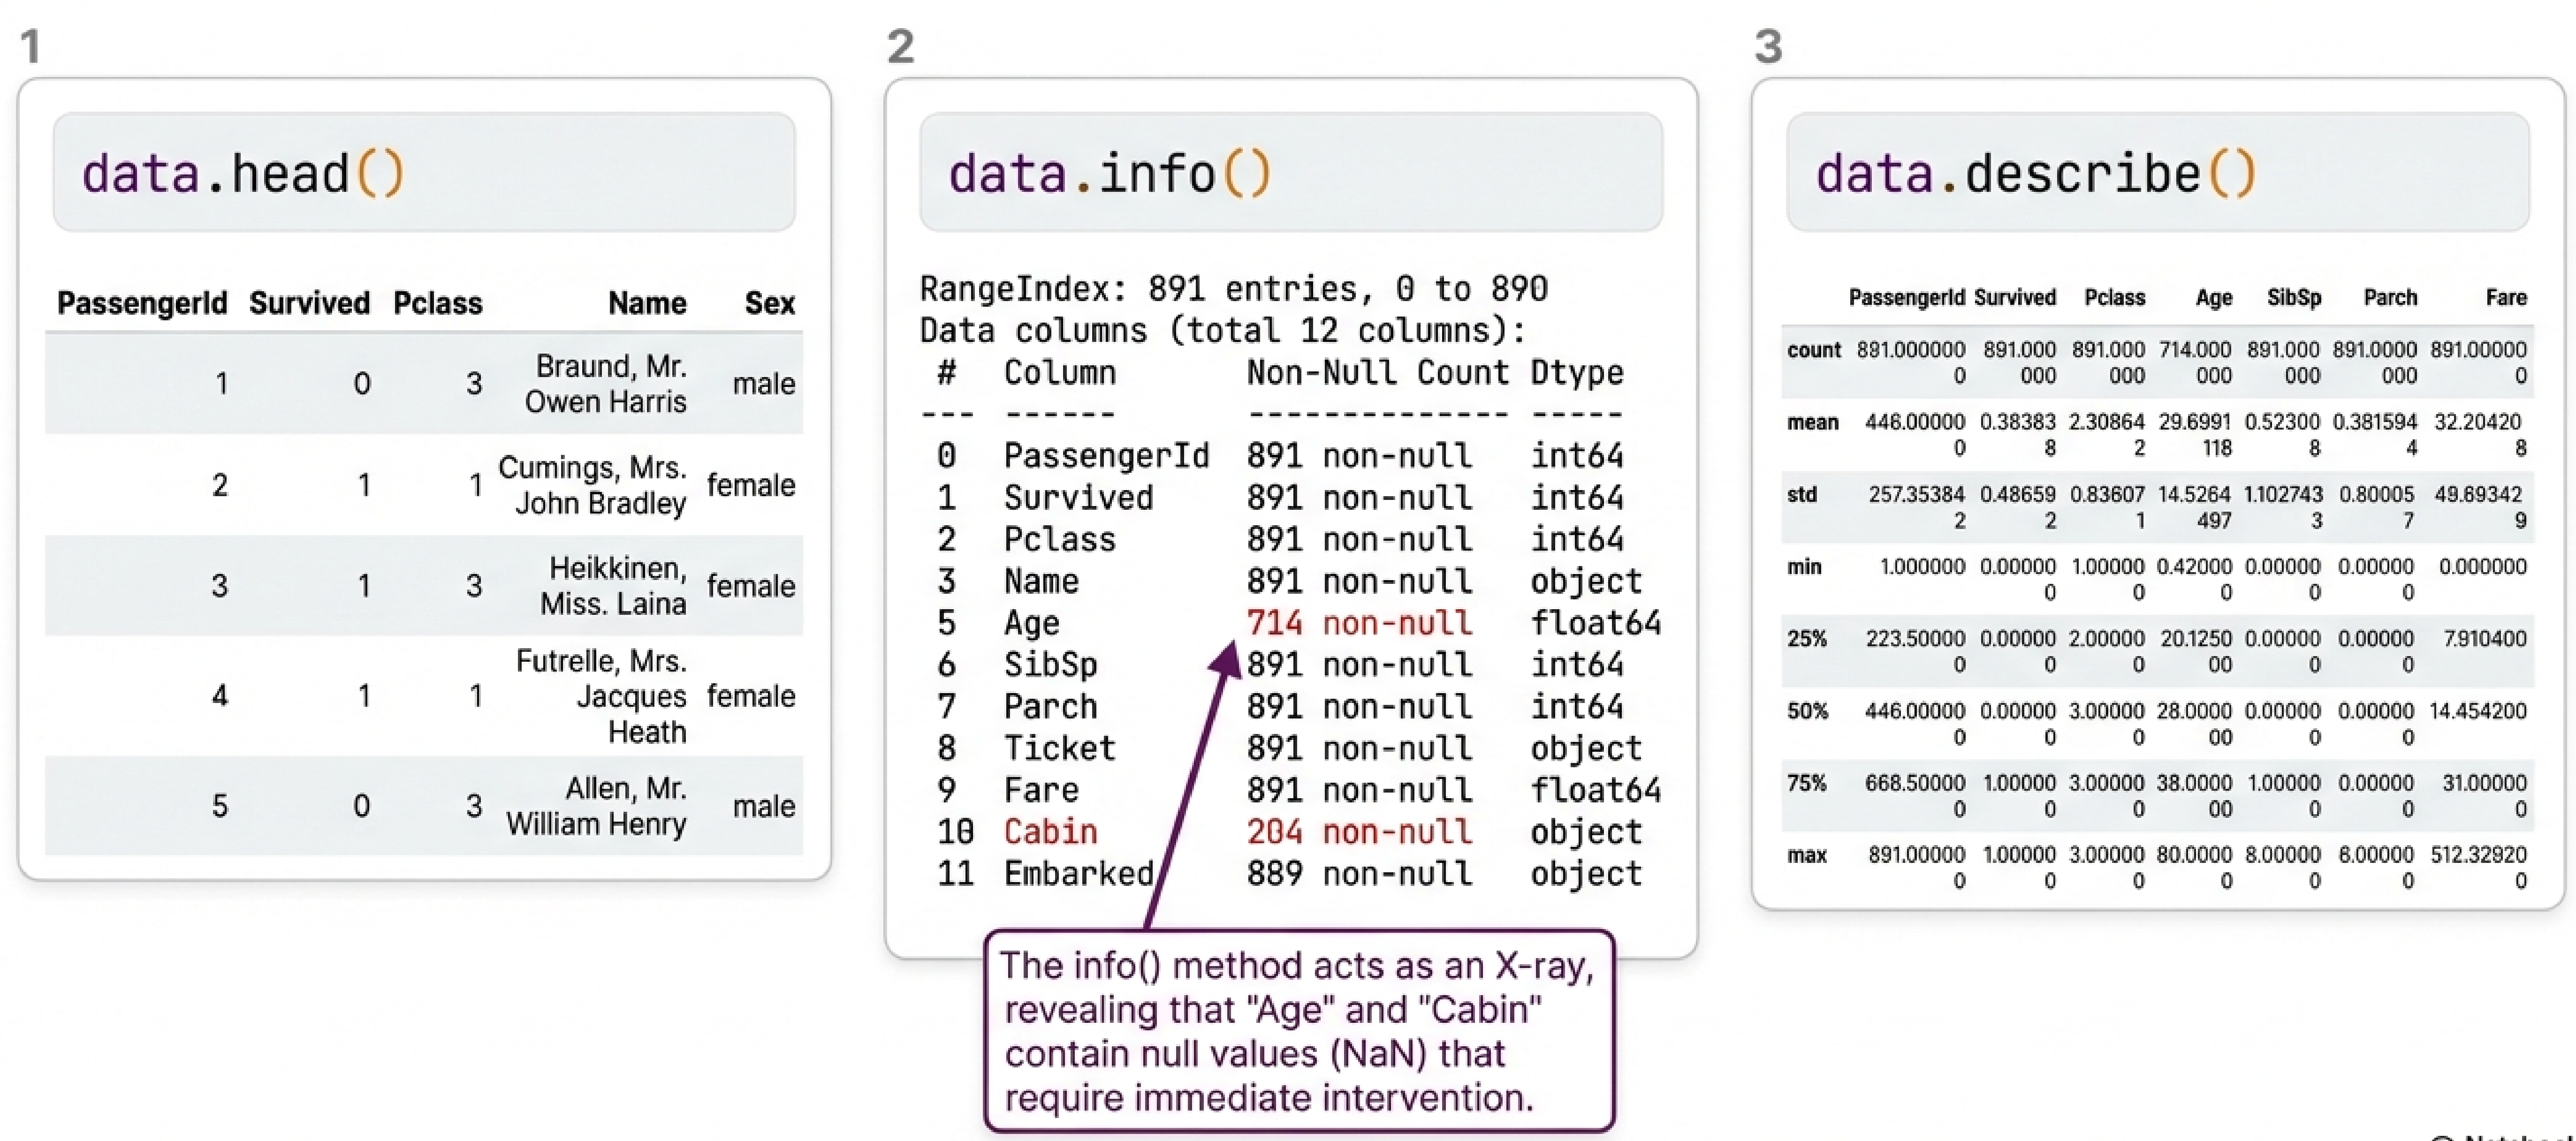
\includegraphics[height=6cm,width=1\textwidth,keepaspectratio]{diagnosis.png}
        % \caption{caption_name}
        \label{fig:diagnosis.png}
    \end{figure}
\end{frame}

\begin{frame}[t]{Where to Study}
    \begin{itemize}
        \item \textbf{Wes McKinney PDF:} Chapter 5 "Getting Started with pandas" (Page 139).
        \item \textbf{Video:} \href{https://www.youtube.com/watch?v=cqBTDb4un-Q}{"Introduction to Data Analysis. Part 1" (Intro section).}
    \end{itemize}
    \note{Глава 5 — база по работе с индексами и осями [15].}
\end{frame}

% --- BLOCK 3: DATA HYGIENE ---
\section{Data Hygiene}

\begin{frame}[t]{Strategies for Missing Data}
    \begin{columns}[T,onlytextwidth]
        \begin{column}{0.25\textwidth}
    \begin{itemize}
        \item Missing values (NaN) are a signal, not just empty space.
        \item Strategy depends on the nature of the data.
    \end{itemize}
    \textbf{Principle:} Handle gaps before they break your model.
        \end{column}
        \begin{column}{0.74\textwidth}
            \vspace*{-0.5cm}
            \begin{figure}[H]
                \centering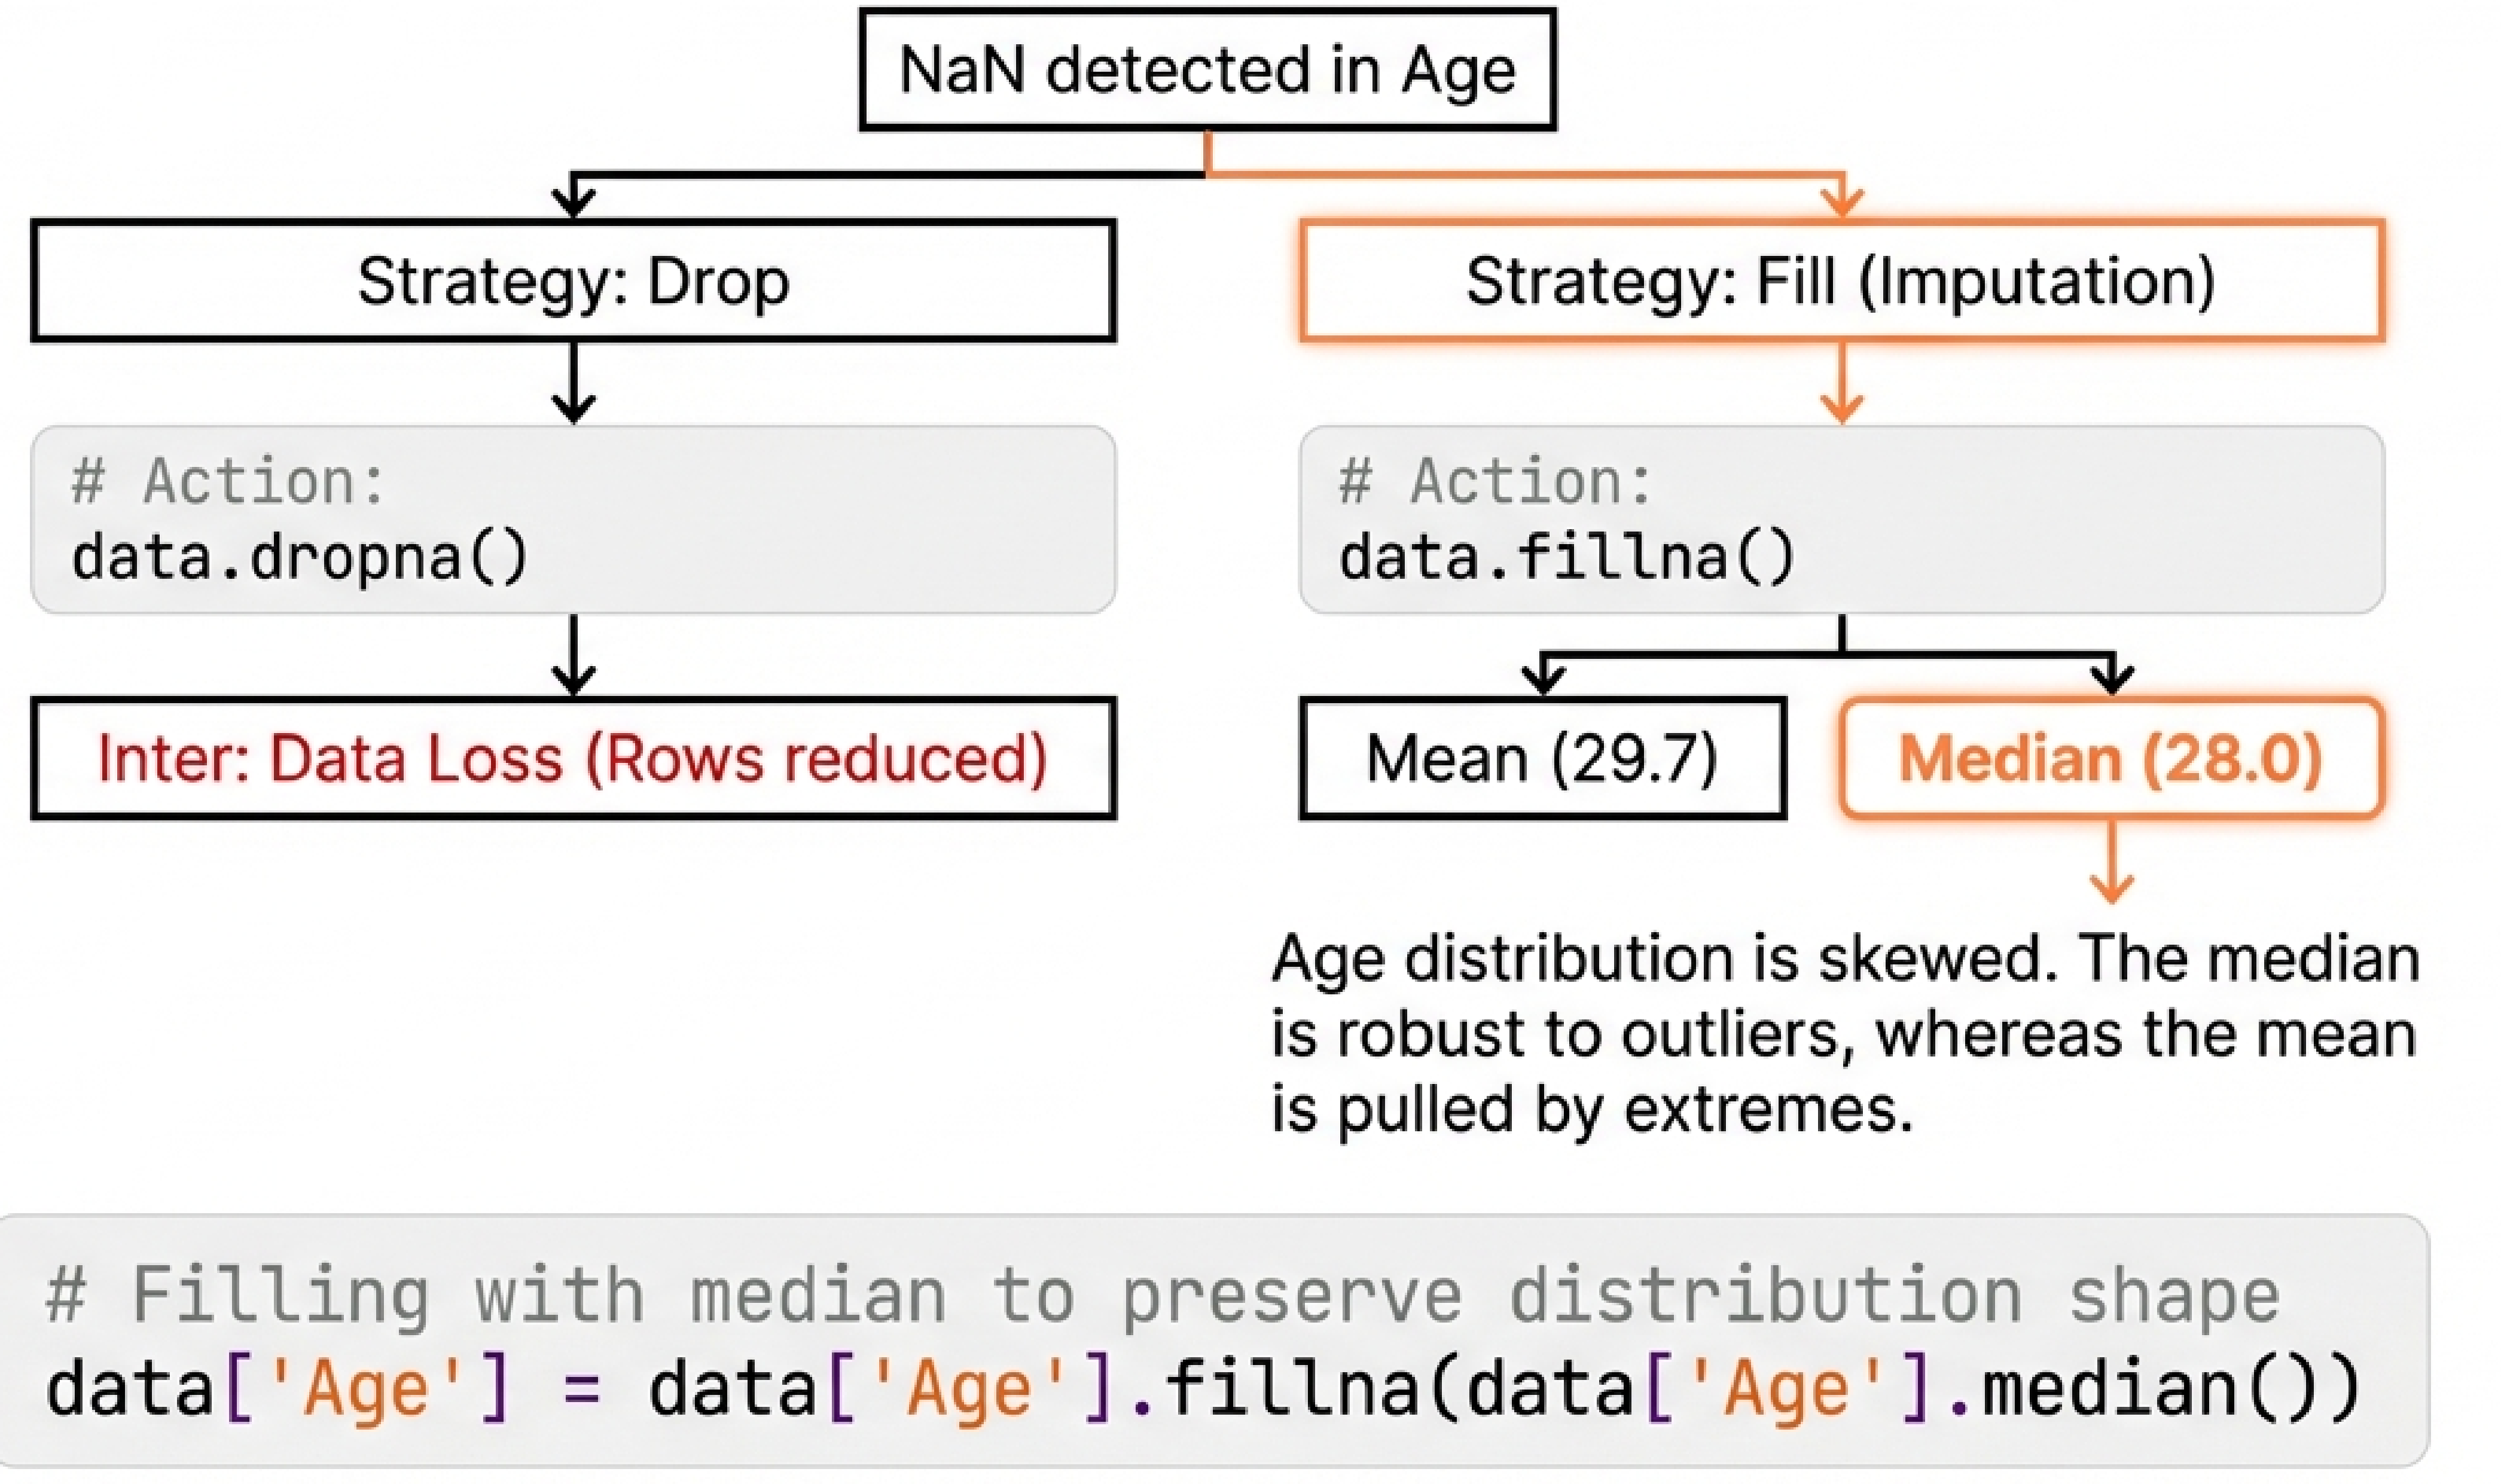
\includegraphics[height=6cm,width=1\textwidth,keepaspectratio]{drop_or_fill.png}
                % \caption{caption_name}
                \label{fig:drop_or_fill.png}
            \end{figure}
        \end{column}
    \end{columns}

    \note{Пропуски в данных — это информация об ошибках сбора. Аналитик должен решить: выкинуть или восстановить [16].}
\end{frame}


\begin{frame}[t]{Visualizing Data Gaps}
    Heatmaps (Seaborn) show the pattern of missingness.
        \begin{figure}[H]
            \centering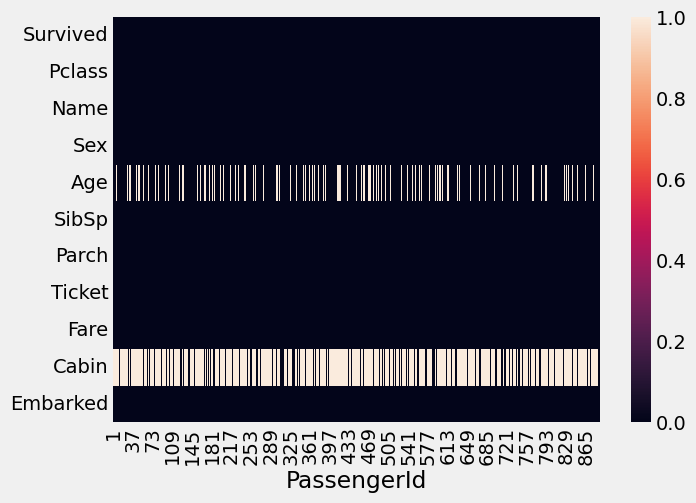
\includegraphics[height=5cm,width=1\textwidth,keepaspectratio]{heatmap.png}
            % \caption{caption_name}
            \label{fig:heatmap.png}
        \end{figure}
    \note{Тепловая карта из семинара наглядно показывает «дыры» в колонках Age и Cabin [17].}
\end{frame}

\begin{frame}[t]{Where to Study}
    \begin{itemize}
        \item \textbf{Wes McKinney PDF:} Chapter 7 "Data Cleaning and Preparation" (Page 214).
        \item \textbf{Video:} \href{https://www.youtube.com/watch?v=PI57kYeODnY}{Introduction to Data Analysis. Part 2" (Preprocessing)}.
    \end{itemize}
    \note{В главе 7 подробно описаны методы fillna и dropna [18].}
\end{frame}

% --- BLOCK 4: EXPLORATORY DATA ANALYSIS (EDA) ---
\section{Exploratory Data Analysis}

\begin{frame}[t]{Concept: Multivariate Analysis}
    \begin{itemize}
        \item Finding linear dependencies between features.
        \item Avoiding redundancy in models.
    \end{itemize}
    \begin{figure}[H]
        \centering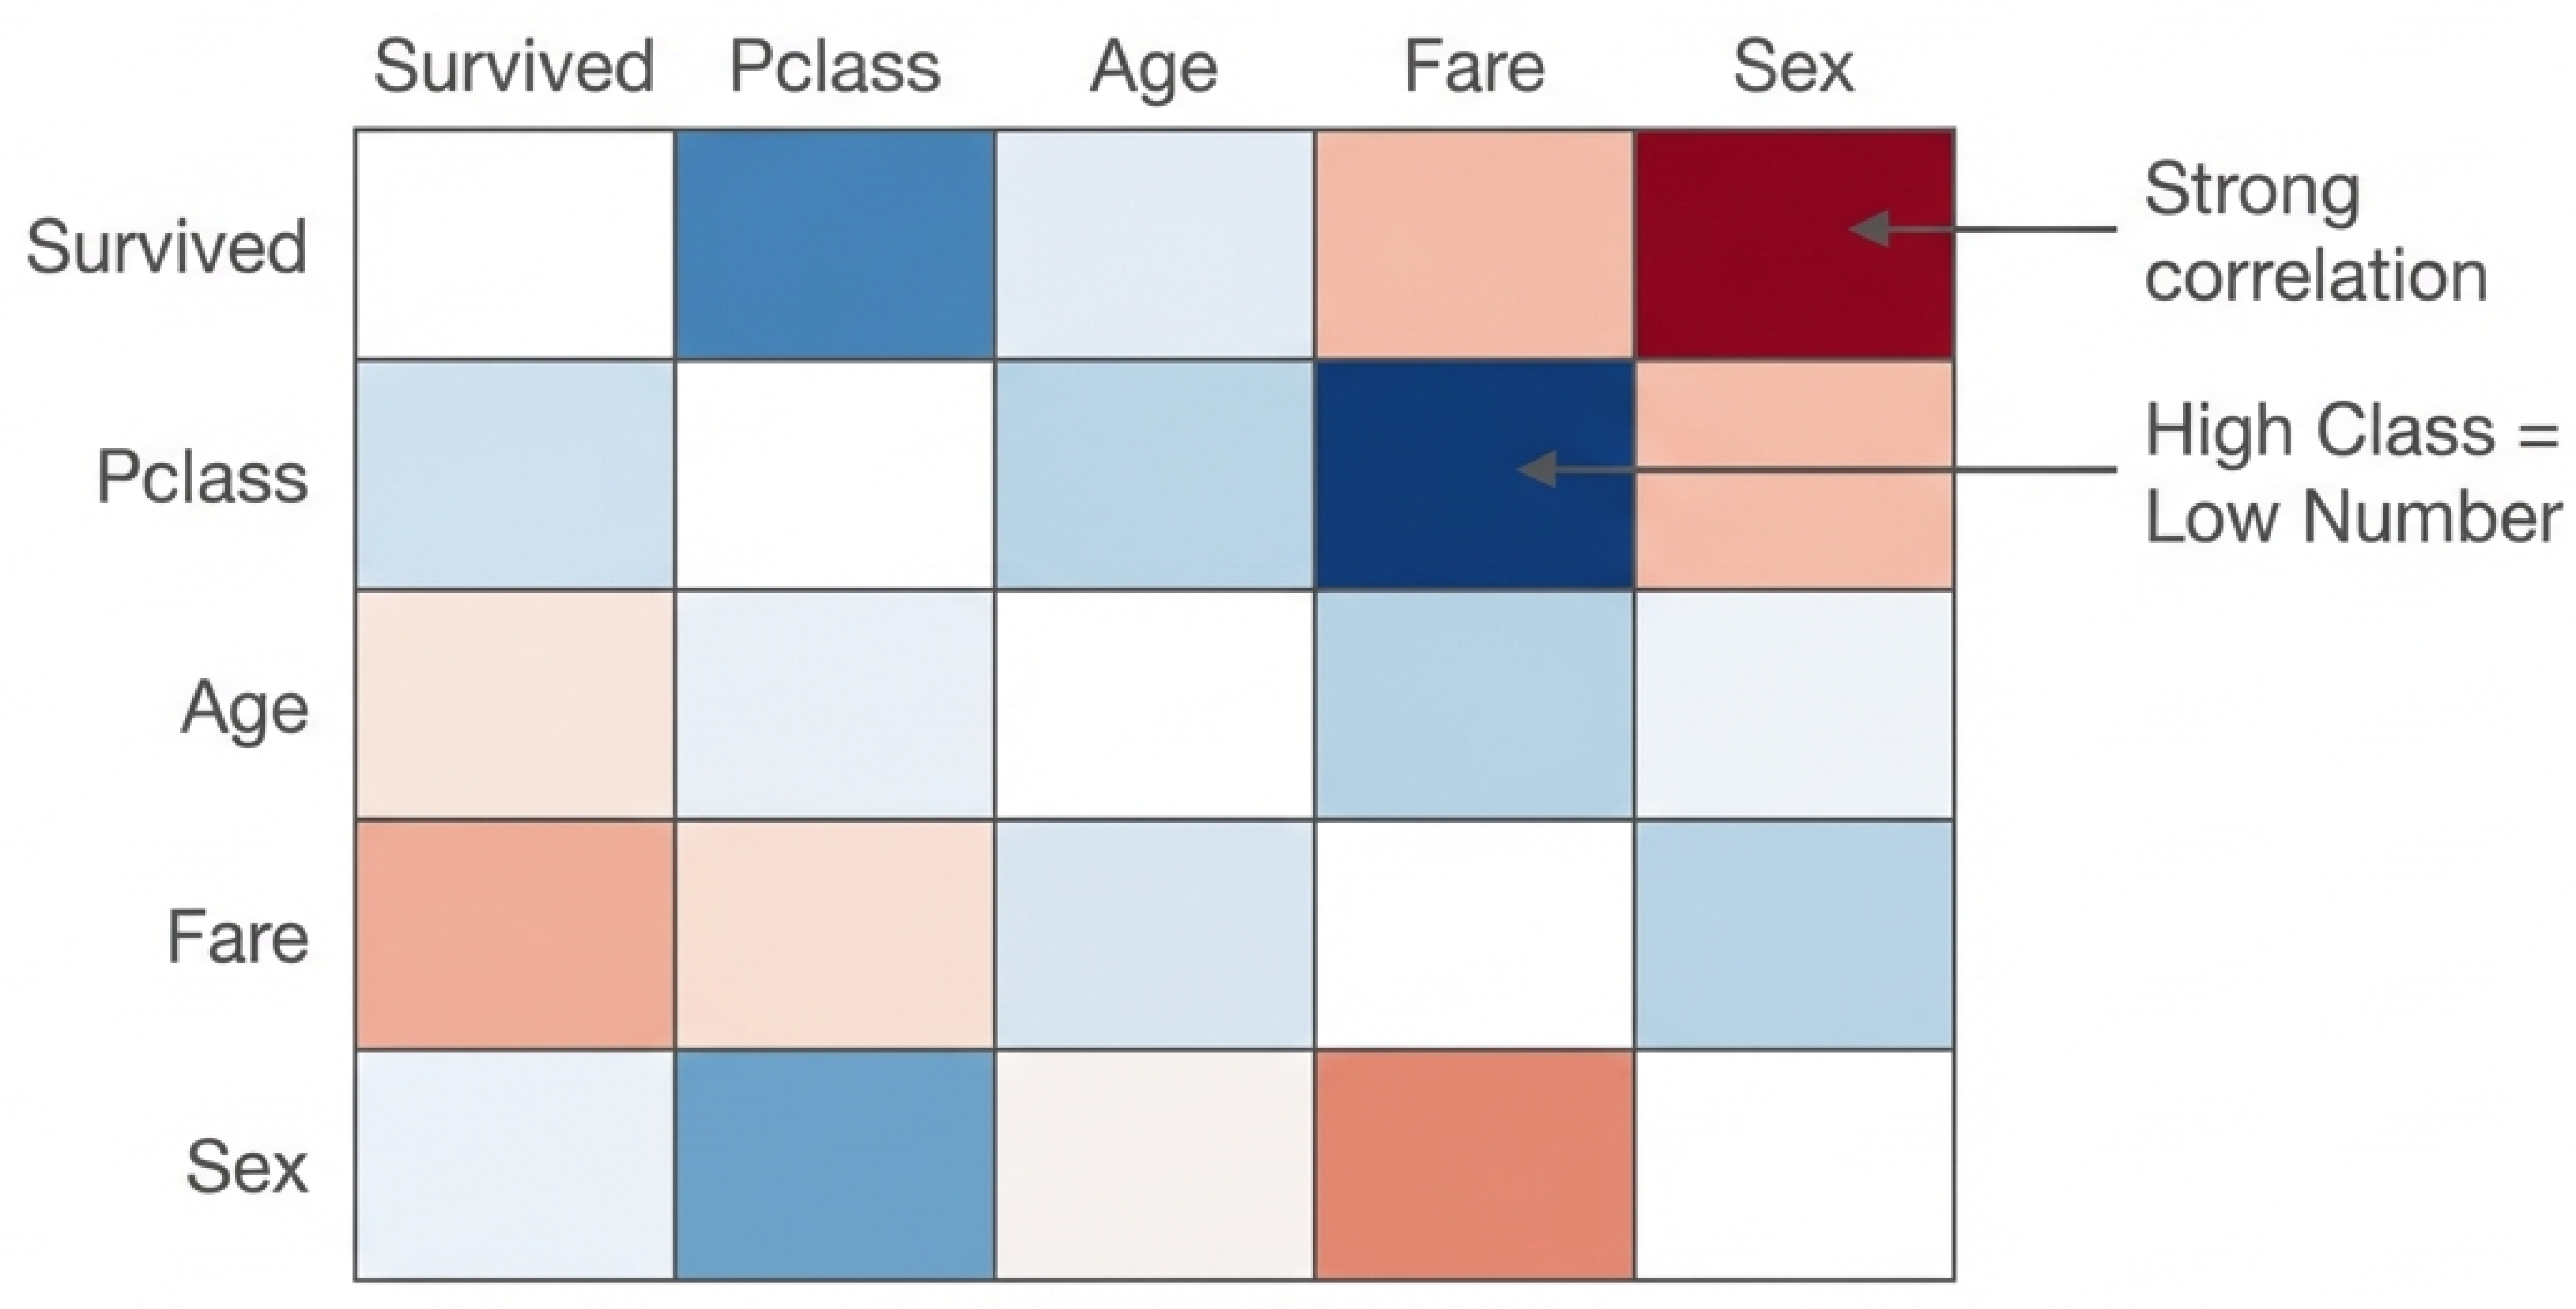
\includegraphics[height=4cm,width=1\textwidth,keepaspectratio]{multivatiate.png}
        % \caption{caption_name}
        \label{fig:multivatiate.png}
    \end{figure}
\end{frame}

\begin{frame}[t]{Aggregation Logic: Split-Apply-Combine}
    \begin{figure}[H]
        \centering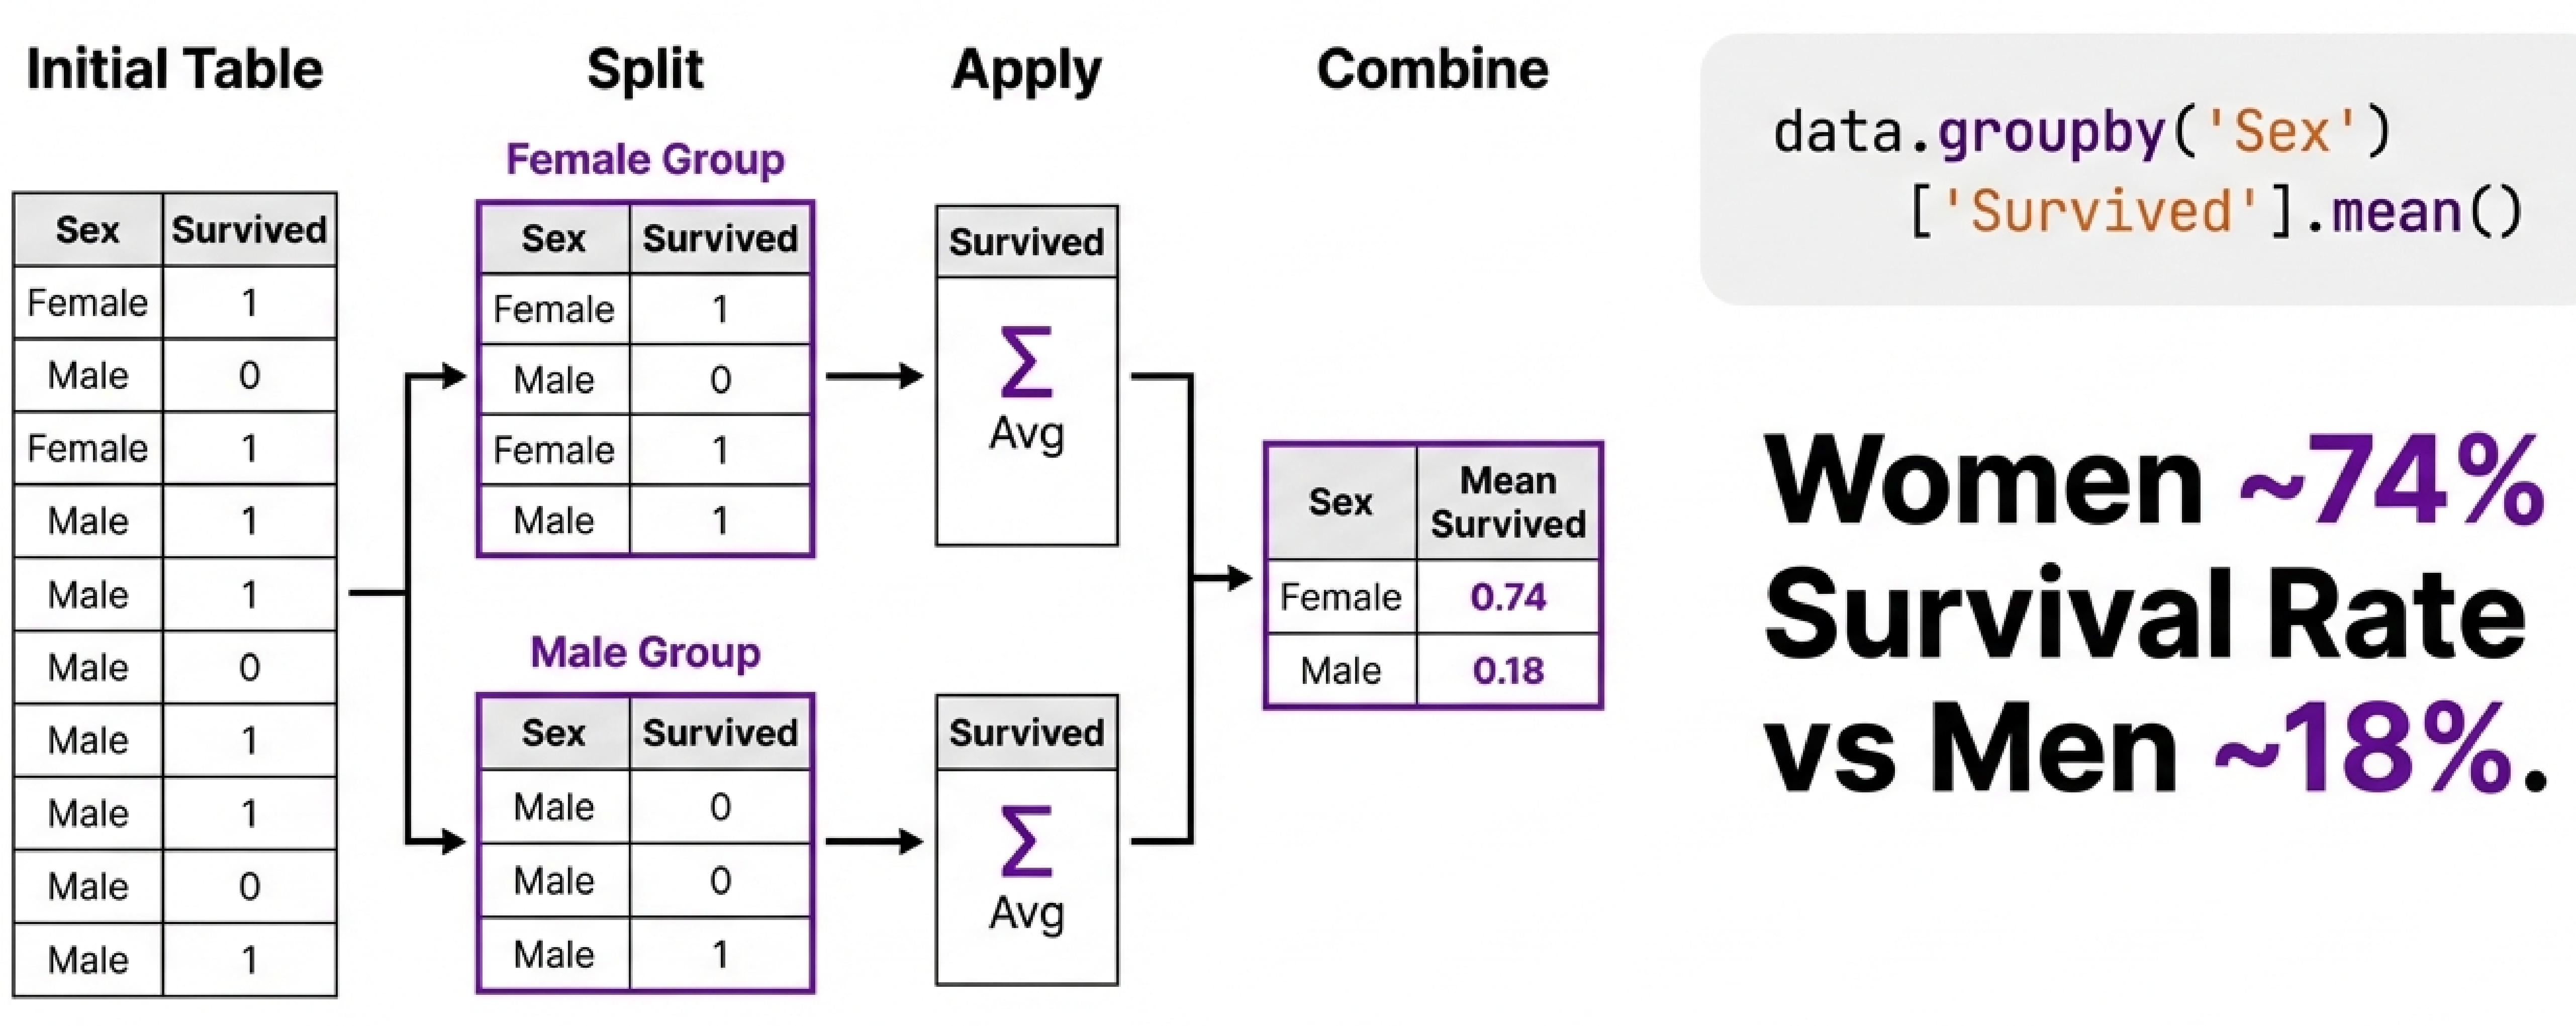
\includegraphics[height=5.5cm,width=1\textwidth,keepaspectratio]{split_apply_combine.png}
        % \caption{caption_name}
        \label{fig:split_apply_combine.png}
    \end{figure}
    \note{Объясните механику GroupBy на примере пола: 74\% выживших женщин против 18\% мужчин [7].}
\end{frame}

\begin{frame}[t]{Univariate Analysis: Distributions}
    \begin{figure}[H]
        \centering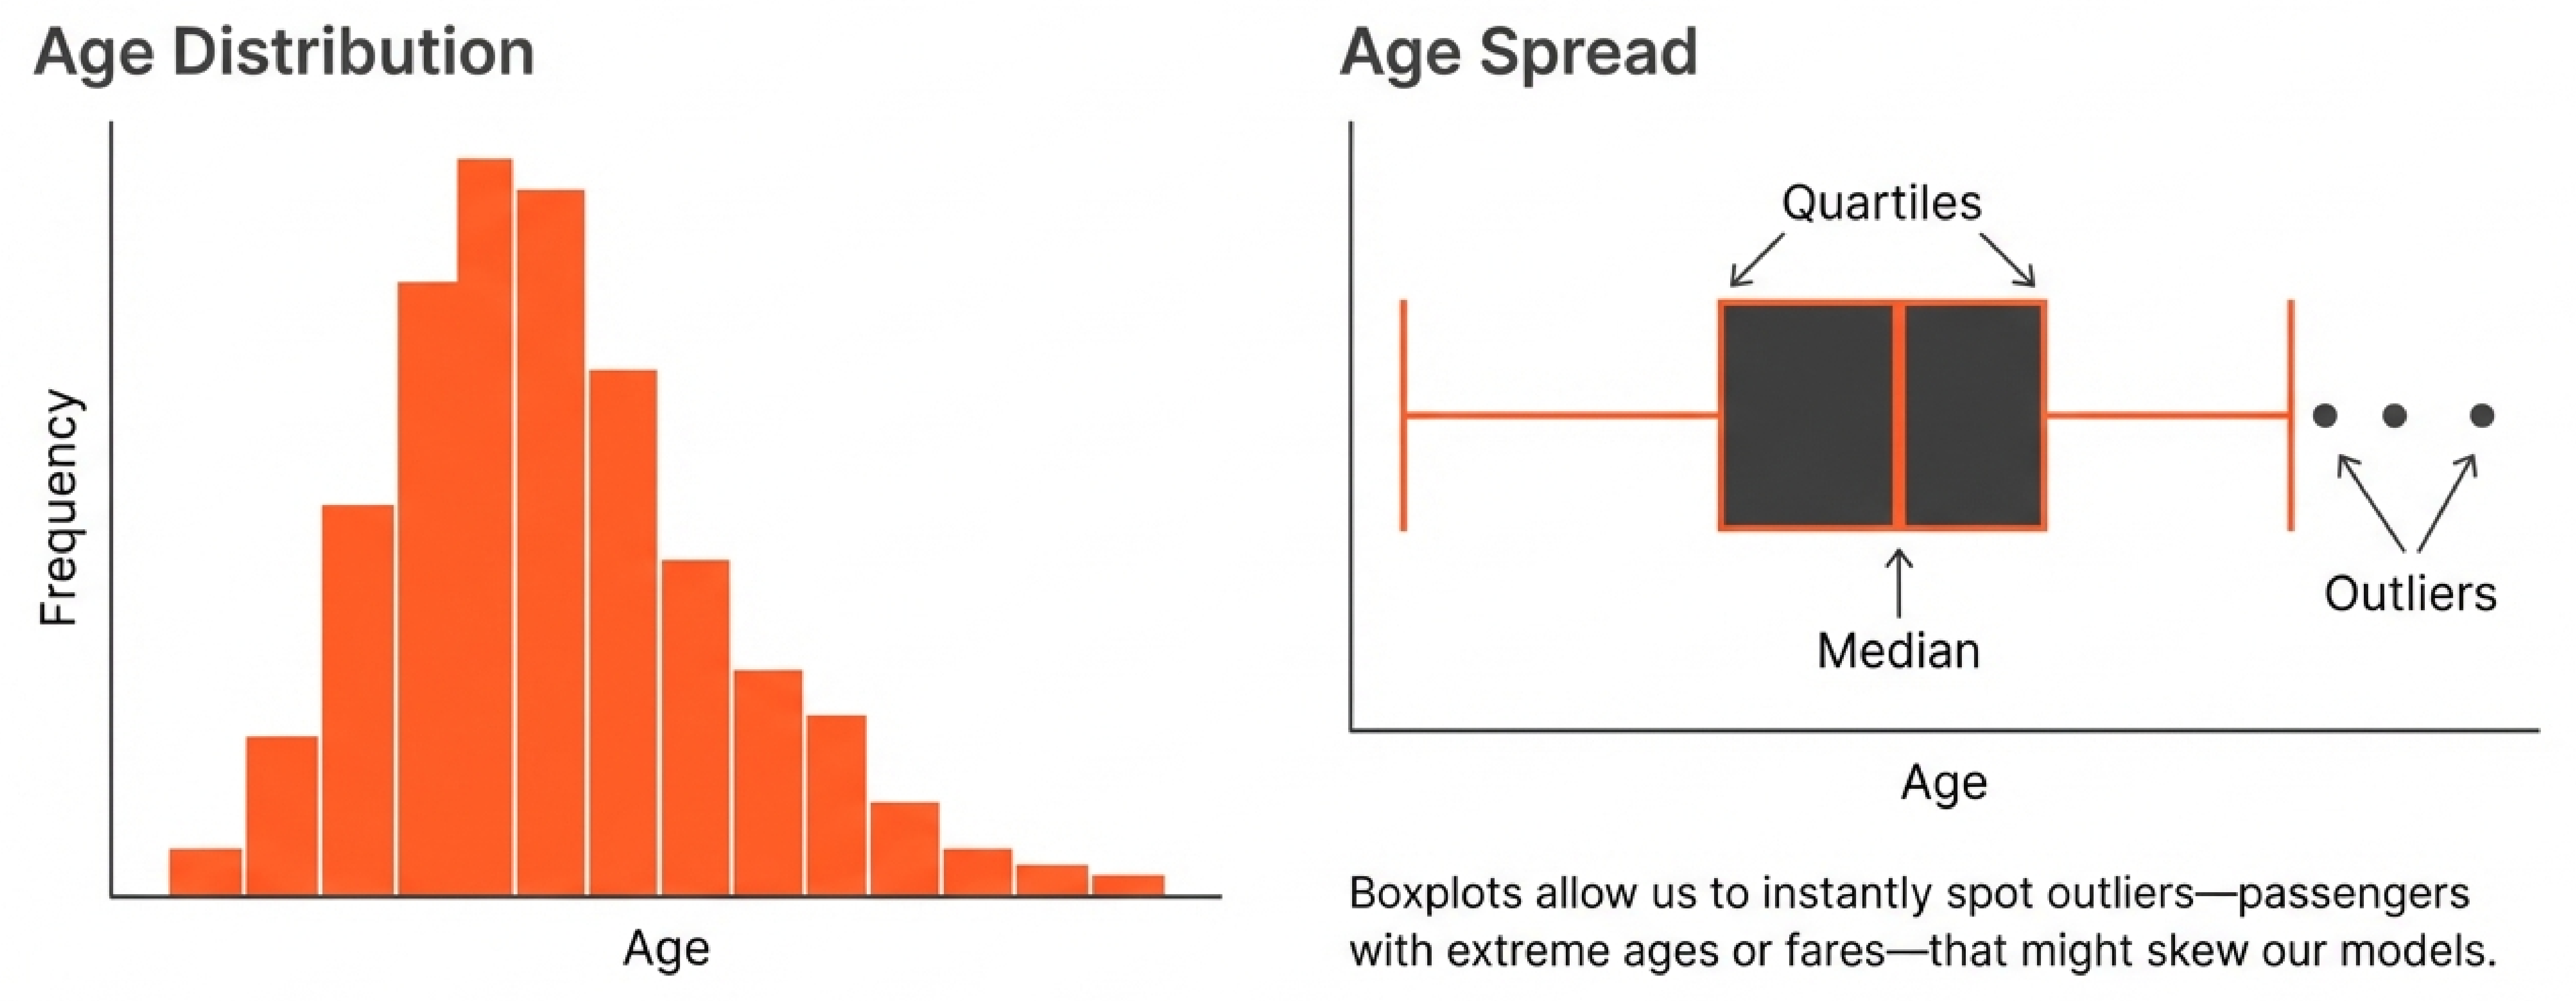
\includegraphics[height=6cm,width=1\textwidth,keepaspectratio]{distribution.png}
        % \caption{/}
        \label{fig:distribution.png}
    \end{figure}
    \note{Сравнение гистограммы и boxplot помогает увидеть разброс возрастов и найти аномалии (выбросы) [8].}
\end{frame}

\begin{frame}[t]{Question-Driven Visualization}
    \begin{itemize}
        \item "Does ticket class affect survival?"
        \item Use Bar charts or Pie charts to answer.
    \end{itemize}
    \note{Напоминайте: мы строим график не ради красоты, а чтобы ответить на конкретный бизнес-вопрос [19].}
\end{frame}

\begin{frame}[t]{Where to Study}
    \begin{itemize}
        \item \textbf{Wes McKinney PDF:} Chapter 9 "Plotting and Visualization" (Page 287).
        \item \textbf{Video:} \href{https://www.youtube.com/watch?v=PI57kYeODnY}{"Introduction to Data Analysis. Part 2" (EDA)}.
    \end{itemize}
    \note{Материалы 9 главы — это стандарт индустрии по визуализации [20].}
\end{frame}

% --- BLOCK 5: ENGINEERING AND ENCODING ---
\section{Engineering and Encoding}

\begin{frame}[t]{Concept: Feature Engineering}
    \begin{itemize}
        \item Creating proxy features for social status and gender.
        \item Transforming unstructured text into meaningful categories.
    \end{itemize}
    \begin{figure}[H]
        \centering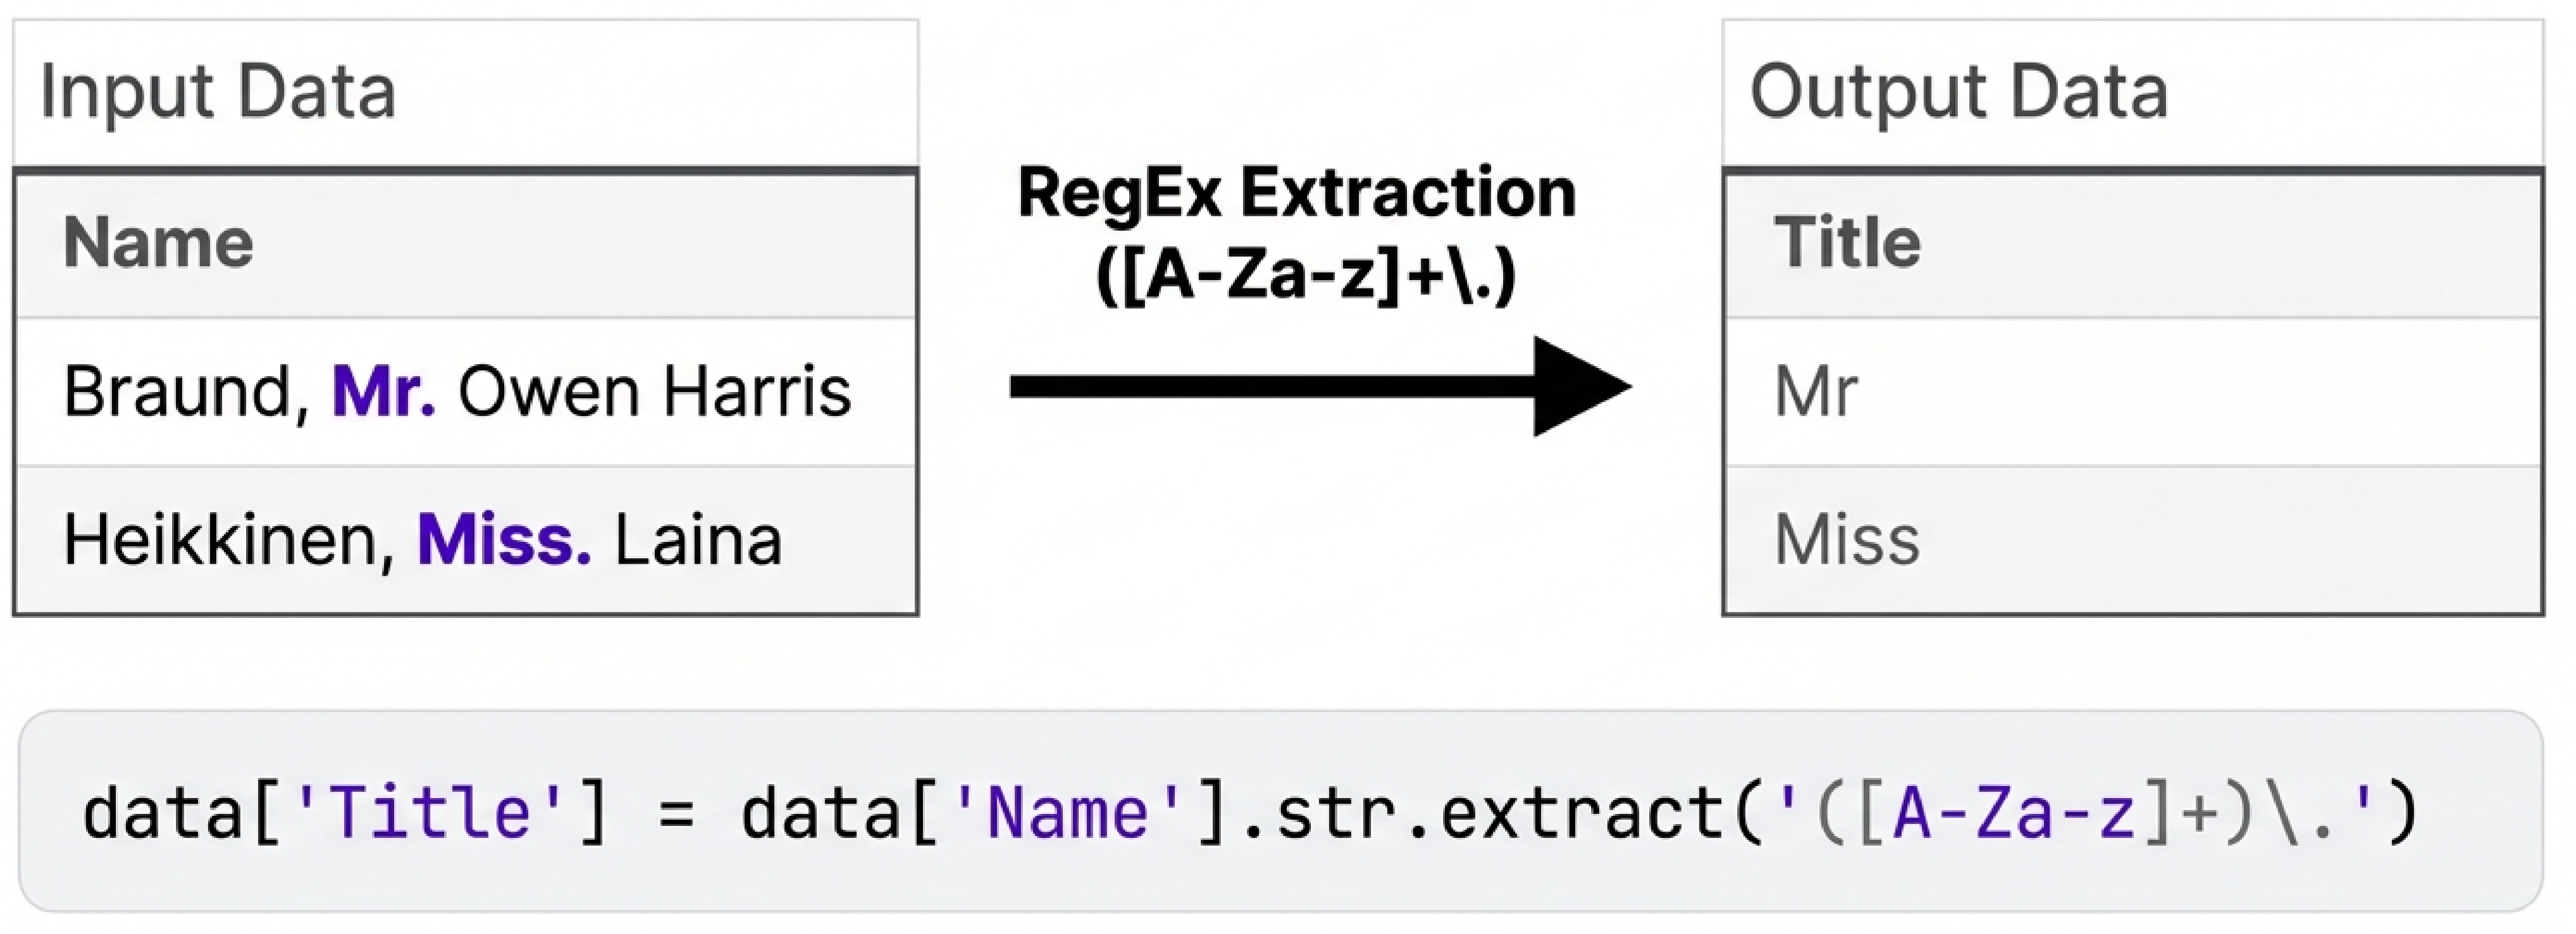
\includegraphics[height=4cm,width=1\textwidth,keepaspectratio]{feature_engineering.png}
        % \caption{caption_name}
        \label{fig:feature_engineering.png}
    \end{figure}
    \note{Покажите, как RegEx превращает бесполезное имя в полезный «Титул» (Mr, Miss), обогащая модель информацией о статусе [6].}
\end{frame}

\begin{frame}[t]{Categorical Encoding}
    \begin{itemize}
        \item Algorithms cannot multiply "City" by a weight.
        \item Numbers are the only language models speak.
    \end{itemize}
    \begin{figure}[H]
        \centering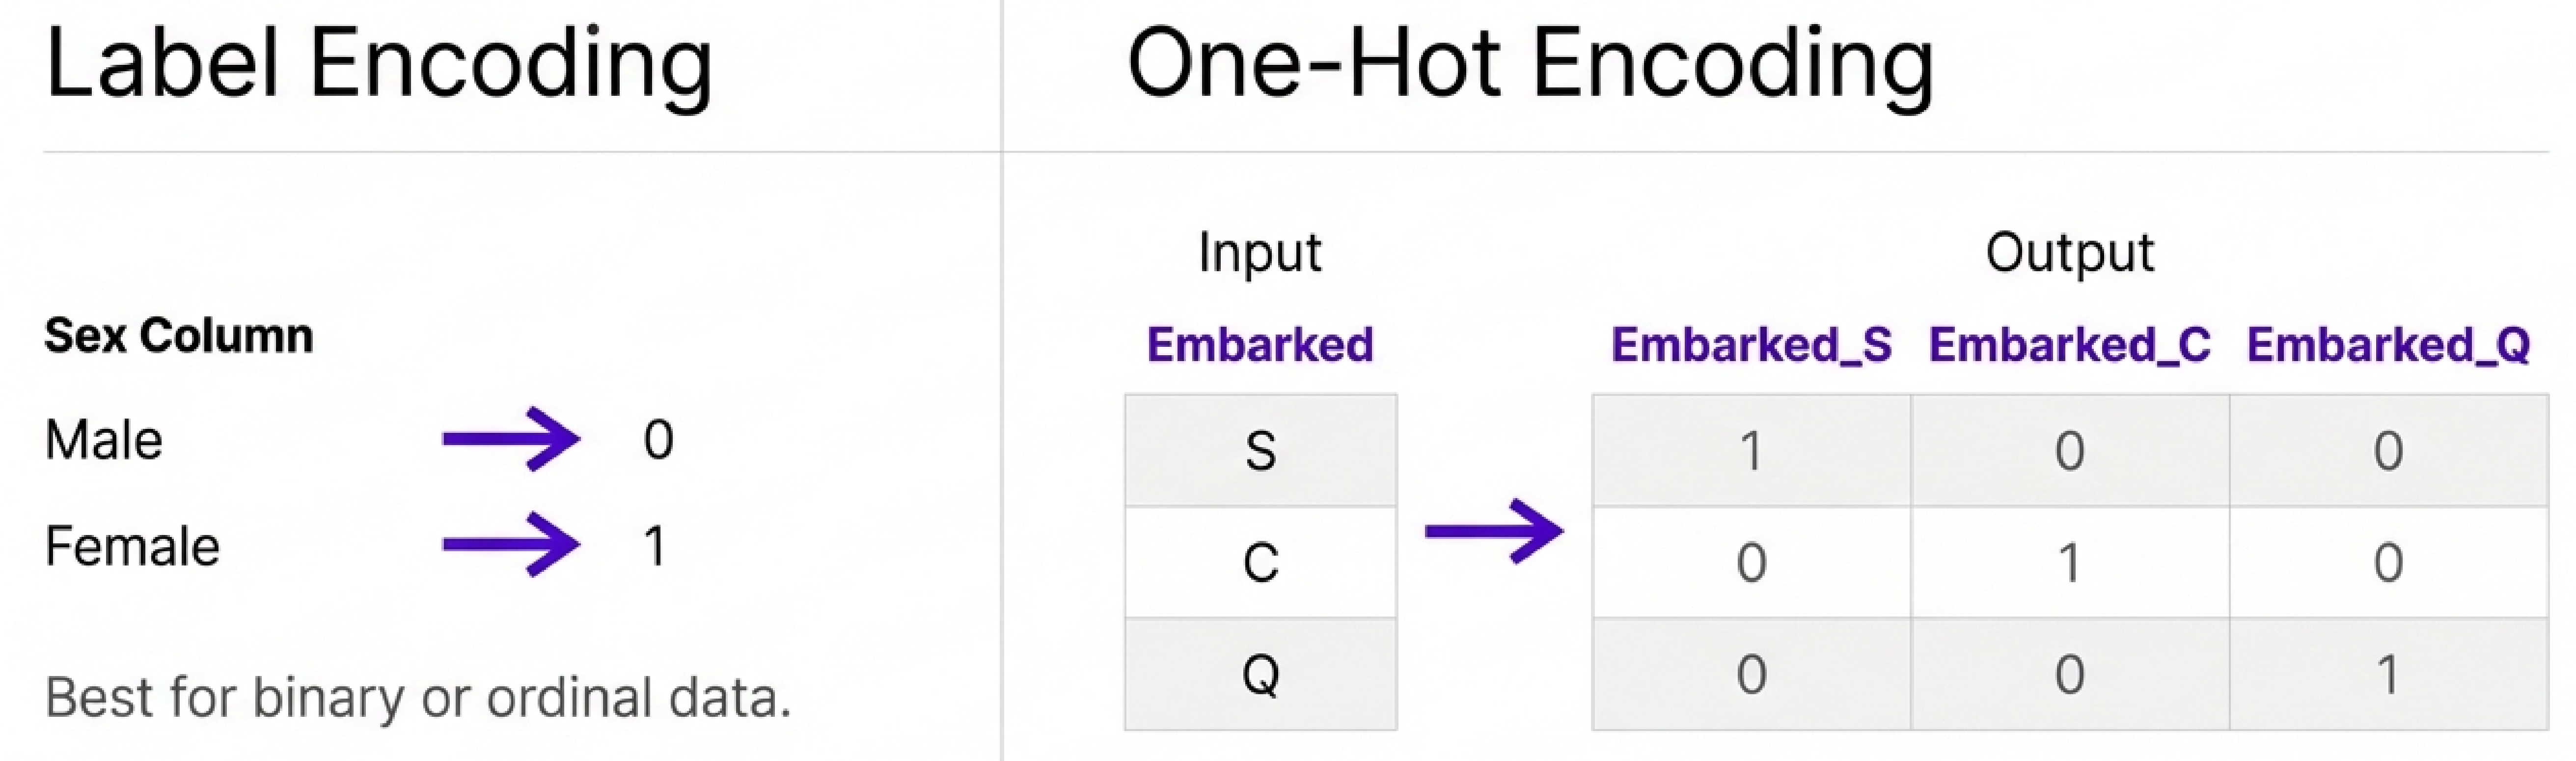
\includegraphics[height=4cm,width=1\textwidth,keepaspectratio]{one_hot.png}
        % \caption{caption_name}
        \label{fig:one_hot.png}
    \end{figure}
    \note{Сравните два подхода: Label Encoding для порядковых данных и One-Hot для равнозначных категорий [10].}
\end{frame}

\begin{frame}[t]{Recap}
    \framesubtitle{Video}
    \vspace*{-0.5cm}
    \begin{figure}[H]
        \href{run:./resources/videoplayback.mp4}{
            \centering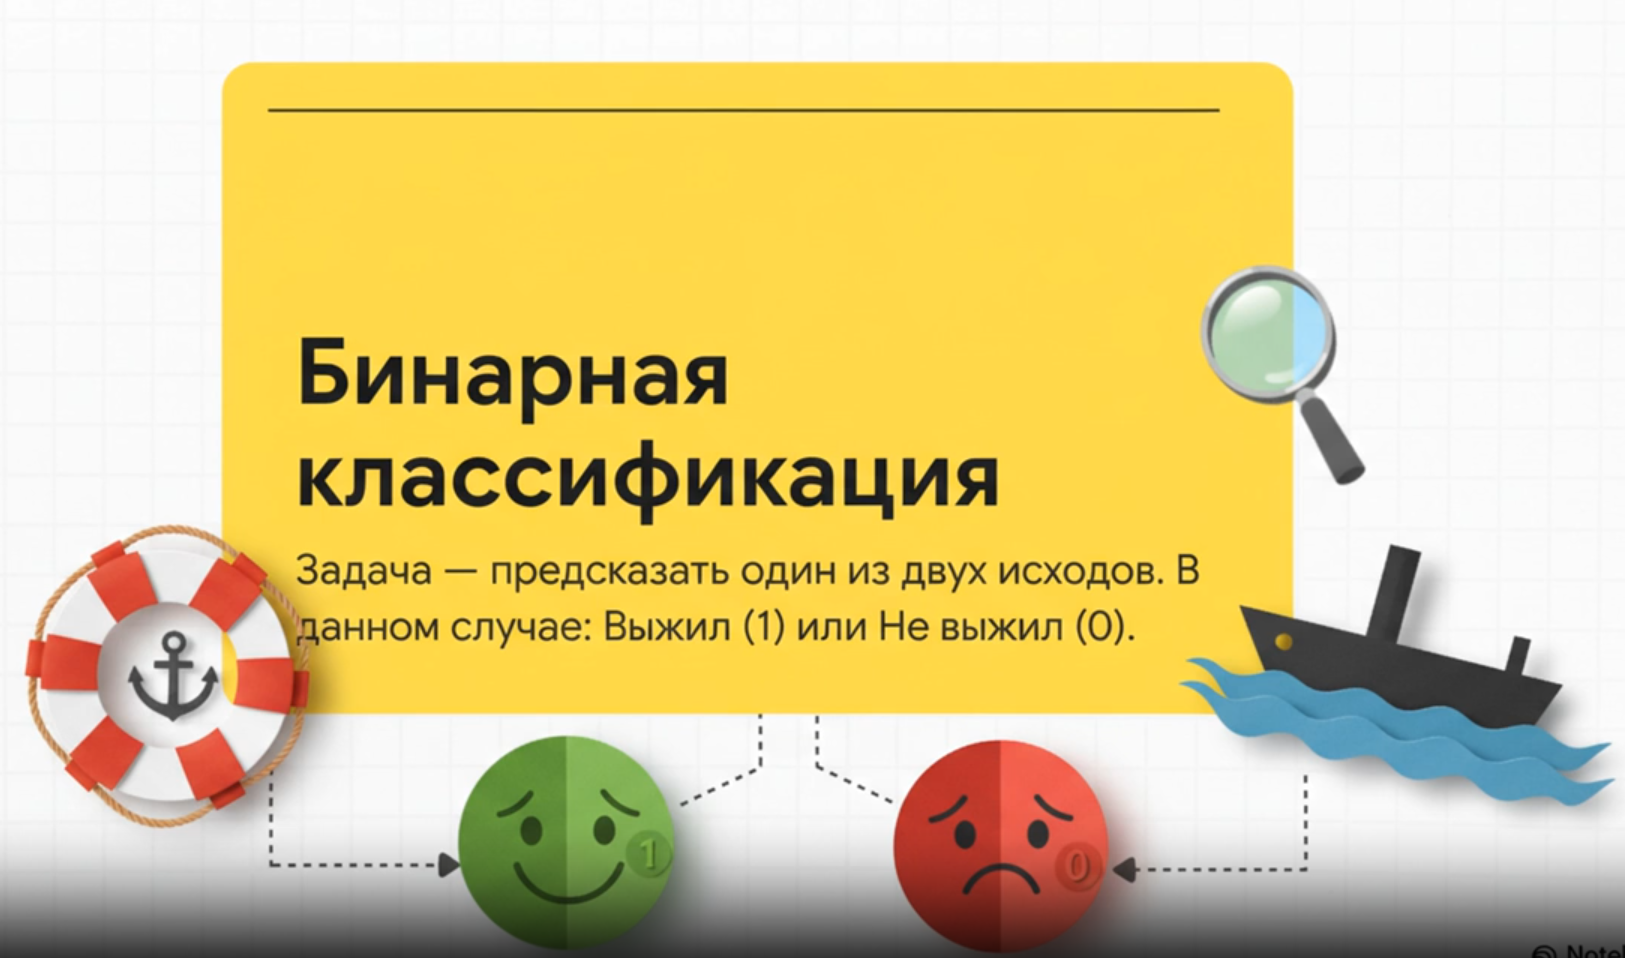
\includegraphics[height=6cm,width=1\textwidth,keepaspectratio]{video_link.png}}
        \label{fig:video_link.png}
    \end{figure}
\end{frame}

\begin{frame}[t]{Reference materials}
\framesubtitle{}
    \begin{itemize}
        \item \href{https://stepik.org/lesson/1909529/step/1?unit=1935583}{Stepik Deep Learning Course, part 3.2}
        \item \href{https://libgen.gl}{<<Python и анализ данных: Первичная обработка данных с применением pandas, NumPy и Jupiter>> Уэс Маккинни}
        \item Jupiter notebooks in <<extra\_materials>> folder.
    \end{itemize}
\end{frame}


\fbckg{fibeamer/figs/last_page.png}
\frame[plain]{}

\end{document}